%
% Kontextfreie Sprachen und pushdown-Automaten
%
% (c) 2019 Prof Dr Andreas Müller, Hochschule Rapperswil
%
\lhead{Kontextfreie Sprachen}
\rhead{Kontextfreie Grammatiken}
\chapter{Stackautomaten und kontextfreie Sprachen\label{chapter-cfl}}
Die regulären Sprachen bilden zwar eine interessante Klasse
von Sprachen mit mathematisch sehr attraktiven Eigenschaften,
doch sind viele praktisch wichtige Sprachen nicht regulär.
Bereits korrekt geschachtelte Klammern können nicht mit einem
DEA erkannt werden.

Ursache ist, dass sich ein DEA nicht
daran ``erinnern'' kann, wieviele Klammern schon geöffnet
worden sind. Um das für beliebig viele Klammern tun zu können,
bräuchte er unendlich viele Zustände (Satz von Myhill-Nerode),
das ist in einem DEA nicht möglich. Dazu ist als Erweiterung
eine Art von Speicher nötig. In diesem Kapitel betrachten
wir Automaten, die mit einem Stack ausgestattet worden sind.

\index{Stack}%
\index{Stackautomat}%
Auch reguläre Ausdrücke sind nicht dazu geeigneet, die Schachtelung
von Klammern auszudrücken. Daher brauchen wir auch für die
regulären Ausdrücke eine Alternative, dies werden die kontextfreien
Grammatiken sein. Es wird sich zeigen, dass die von Stackautomaten
akzeptierten Sprachen auch mit einer kontextfreien Grammatik erzeugt
werden können, wir haben also eine ähnliche Situation wie
bei DEAs und regulären Ausdrücken. So entsteht die neue
Kategorie der kontextfreien Sprachen.
\index{Sprache!kontextfreie}%
Natürlich werden auch kontextfreie Sprachen nicht alles
abdecken, so dass wir wieder ein Kriterium brauchen, mit dem
man entscheiden kann, ob eine Sprache kontextfrei ist. Wir
werden auch für kontextfreie Sprachen
ein Pumping Lemma finden.

%
% grammatik.tex -- Grammatik
%
% (c) 2019 Prof Dr Andreas Müller, Hochschule Rapperswil
%
\section{Kontextfreie Sprachen}
\rhead{Kontextfreie Sprachen}
\subsection{Kontextfreie Grammatiken}
Reguläre Sprachen werden dadurch definiert, dass die Zeichen
eines Wortes von links nach rechts gelesen werden, und nach jedem
Zeichen entschieden werden kann, ob das Wort akzeptabel ist.
Der Fokus liegt also auf der Analyse des Strings, und genau dies
macht das Überprüfen der korrekten Schachtelung von Klammern
schwierig.

\index{Ausdrücke!arithmetische}%
Für Klammern ist man sich jedoch meistens eine andere Vorgehensweise
gewohnt.
Wenn man arithmetische Ausdrücke aufbaut, sagt man zum
Beispiel: ``Wenn man die Summe $a+b$ mit $c$ multiplizeren will,
dann {\em muss man $a+b$ in Klammern setzen}''.
Klammern werden also immer paarweise gesetzt, und man baut den
Ausdruck sozusagen von innen nach aussen auf.

Wir möchten diese Idee ein Stück weit formalisieren.
Das Ziel ist,
Wörter aus den Zeichen {\tt (} und {\tt )} aufzubauen, die korrekte
Klammerausdrücke sind.
Dazu können wir bereits bekannte korrekte
Klammerausdrücke aneinanderhängen, oder wir können einen bereits
bekannten korrekten Ausdruck ``einklammern''.
Schreiben wir $A$
für einen Klammerausdruck, bedeutet das, dass wir $A$ gemäss
folgender Regeln umformen können:
\begin{align*}
A&\to AA\\
A&\to {\tt (}A{\tt )}
\end{align*}
Dabei ist auf der rechten Seite der ersten Regel gemeint, dass wir zwei beliebige
Ausdrücke nehmen können, sie müssen nicht identisch sein.
Allerdings
fehlt in diesen Regeln noch ein Anfang, bis jetzt können wir überhaupt
keine Wörter produzieren.
Dazu nehmen wir noch eine Regel $A\to\varepsilon$
hinzu, die besagt, dass das leere Wort auch ein akzeptabler
Klammerausdruck ist.
Die Regeln
\begin{align}
A&\to\varepsilon       \label{regeln-beispiel-1}\\
A&\to AA               \label{regeln-beispiel-2}\\
A&\to {\tt (}A{\tt )}  \label{regeln-beispiel-3}
\end{align}
erzeugen in diesem Sinne alle korrekt geschachtelten Klammerausdrücke.

Der Buchstabe $A$ steht offenbar nicht immer für das gleiche, 
er ist Platzhalter für einen korrekten Klammerausdruck.
Wir nennen $A$ eine Variable.
Dagegen stehen die Zeichen {\tt (} und {\tt )} nur für sich selbst, sie
können nicht weiter ersetzt werden, sie heissen Terminalsymbole.

Damit sind wir bereit für die formale Definition einer kontextfreien
Grammatik.
\begin{definition}
\index{Grammatik!kontextfreie}%
Eine kontextfreie Grammatik ist ein Quadrupel $(V,\Sigma,R,S)$ mit
\begin{compactenum}
\index{Variable}%
\item $V$ ist eine endliche Menge von Variablen.
\index{Terminalsymbol}%
\item $\Sigma$ ist eine endliche Menge von Zeichen, disjunkt zu $V$,
auch genannt die Terminalsymbole.
\item $R$ ist eine Menge von Regeln, eine Regel besteht aus einer
Variable und einer Kette von Variablen und Terminalsymbolen, geschrieben
in der Form $A\to BC{\tt x}$, wobei rechts eine beliebige Folge von
Variablen (in diesem Fall $A$ und $B$) und Terminalsymbolen (in diesem Fall
\texttt{x}) stehen kann.
\index{Regel!einer kontextfreien Grammatik}%
\item $S\in V$ ist die Startvariable.
\index{Startvariable}%
\end{compactenum}
\end{definition}
Im Beispiel ist $V=\{A\}$, $\Sigma=\{{\tt (},{\tt )}\}$, $S=A$ und
$R$ enthält genau drei Regeln (\ref{regeln-beispiel-1}) bis
(\ref{regeln-beispiel-3}).

Zur Abkürzung erlauben wir, Regeln mit der gleichen Variablen
auf der linken Seite des Pfeils mit einem Vertikalstrich als
Verknüpfungszeichen auf der rechten Seite zu schreiben, zu lesen
als ``oder'':
\[
A \to \varepsilon\;|\; AA\;|\; {\tt (}A{\tt )}.
\]

Der Name ``kontextfrei'' rührt daher, dass es bei der Anwendung
der Regeln nicht auf den Kontext ankommt, in dem eine Variable
auf der linken Seite des Pfeils~$\rightarrow$ vorkommt.
Regeln der Form 
\[
{\tt a}A\to AA, \qquad {\tt bA}\to BB,
\]
sogenannte kontextsensitive Regeln,
\index{kontextsensitiv}%
würden dagegen ausdrücken, dass die Umwandlung der Variablen $A$
unterschiedlich zu erfolgen hat, wenn ihr verschiedene Zeichen
vorangehen.
In diesem Fall käme es auf den Kontext an.
Solche Regeln sollen jedoch nicht zugelassen sein.

\subsection{Kontextfreie Sprachen}
Eine Grammatik erzeugt eine Sprache auf die folgende Weise.
Auf die Startvariable werden beliebige Regeln angewendet,
bis keine Variablen mehr vorhanden sind, jetzt steht nur noch
eine Kette von Terminalsymbolen da.
Dies wollen wir wie folgt formalisieren.

\begin{definition}
\index{Regel!erzeugtes Wort}%
\index{Ableitung}%
Falls $A\to w$ eine Regel einer Grammatik $G$ ist, sagt man
dass die Regel aus $uAv$ den String $uwv$ erzeugt,
geschrieben $uAv\Rightarrow uwv$.
Man sagt, $v$ lässt sich aus
$u$ ableiten, wenn es eine Folge $u_1,\dots,u_n$ gibt mit
\[
u\Rightarrow u_1\Rightarrow u_2\Rightarrow\dots\Rightarrow u_n\Rightarrow v,
\]
auch geschrieben als $u\overset{*}{\Rightarrow} v$
\end{definition}

\begin{beispiel}
Als Beispiel sei das Wort \texttt{(()())} aus der Grammatik
(\ref{regeln-beispiel-1})
bis
(\ref{regeln-beispiel-2})
für die Klammerausdrücke abgeleitet:
\begin{align*}
A
&\xrightarrow{\text{(\ref{regeln-beispiel-3})}} \texttt{(} A \texttt{)}
 \xrightarrow{\text{(\ref{regeln-beispiel-2})}} \texttt{(} AA \texttt{)}
 \xrightarrow{\text{(\ref{regeln-beispiel-3})}} \texttt{((} A\texttt{)}A \texttt{)}
 \xrightarrow{\text{(\ref{regeln-beispiel-3})}} \texttt{((} A\texttt{)(}A \texttt{))}
 \xrightarrow{\text{(\ref{regeln-beispiel-1})}} \texttt{((} \texttt{)(}A \texttt{))}
 \xrightarrow{\text{(\ref{regeln-beispiel-1})}} \texttt{((} \texttt{)(} \texttt{))}
\end{align*}
Die Reihenfolge der Regelanwendung ist nicht eindeutig.
\end{beispiel}

\begin{definition}
\index{Sprache!von einer CFG erzeugte}%
Die Menge aller Wörter, die von einer kontextfreien Grammatik 
$G$ erzeugt werden können wir mit
\[
L(G)=\{w\in\Sigma^*\;|\; S\overset{*}{\Rightarrow} w\}
\]
bezeichnen.
\end{definition}

Zu jeder kontextfreien Grammatik gibt es also eine Sprache bestehend aus
den von der Grammatik produzierten Wörtern.
Die kontextfreien Sprachen sind die Sprachen, die auf diese Weise entstehen.

\begin{definition}
\index{kontextfreie Sprache}%
\index{Sprache!kontextfrei}%
Eine Sprache $L$ heisst {\em kontextfrei}, wenn es eine kontextfreie
Grammatik $G$ gibt derart, dass $L=L(G)$.
\end{definition}

\subsection{Beispiele}
\subsubsection{Natürliche Zahlen}
Natürliche Zahlen sind Wörter über dem Alphabet $\Sigma=\{
{\tt 0},
{\tt 1},
{\tt 2},
{\tt 3},
{\tt 4},
{\tt 5},
{\tt 6},
{\tt 7},
{\tt 8},
{\tt 9}\}$, welche von den Grammatikregeln
\begin{align*}
N&\to Z\\
 &\to NZ\\
Z&\to {\tt 0}\;|\;\dots \;|\;{\tt 9}
\end{align*}
erzeugt werden.

Diese Grammatik hat aber den Mangel, dass sie auch Zahlen
mit führenden Nullen erlaubt.
Diese könnten dadurch entfernt
werden, dass wir eine weitere Variable für zulässige
Anfangsziffern einführen.
Die Bezeichnung der Variablen mit einzelnen Buchstaben wird jetzt
bereits etwas unübersichtlich, wir schreiben die Grammatik daher neu
so:
\begin{align*}
\textsl{zahl}           &\to\textsl{nichtnullziffer}\; \textsl{ziffernfolge} \\
                        &\to\textsl{ziffer}\\
\textsl{ziffernfolge}   &\to \textsl{ziffernfolge}\; \textsl{ziffer}\\
                        &\to \textsl{ziffer}\\
\textsl{ziffer}         &\to \texttt{0}\; |\; \textsl{nichtnullziffer}\\
\textsl{nichtnullziffer}&\to \texttt{1}\;|\;\texttt{2}\;|\;\dots\;|\;\texttt{9}
\end{align*}
Damit ist auch gleich der Fall einer einzelnen Null abgehandelt, denn eine
solche ist ja eine \textsl{ziffer}, und eine \textsl{zahl} kann auch eine
einzelne Ziffer sein.

\subsubsection{Einfache arithmetische Ausdrücke}
\index{Ausdrücke!arithmetische}%
\index{expression-term-factor Grammatik}%
Auch arithemtische Ausdrücke können mit einer
Grammatik erzeugt werden.
Da die Zahl der Variablen schnell grösser
wird, werden wir im Folgenden auch längere Variablennamen zulassen.
Als Alphabet verwenden wir
$\Sigma=\{{\tt 0},\dots,{\tt 9},{\tt +},{\tt *},{\tt (}, {\tt )}\}$.
Die Startvariable drückt aus, was erzeugt werden soll, in diesem Fall
ein Ausdruck, also nennen wir sie \textsl{expression}.
Folgende Grammatik
erzeugt die arithmetischen Ausdrücke:
\begin{align*}
\textsl{expression} &\to \textsl{expression}\;{\tt +}\;\textsl{term}\\
                    &\to \textsl{term}\\
\textsl{term}       &\to \textsl{term}\;{\tt *}\;\textsl{factor}\\
                    &\to \textsl{factor}\\
\textsl{factor}     &\to {\tt (}\textsl{expression}{\tt )}\\
                    &\to N\\
N                   &\to Z\\
                    &\to NZ\\
Z                   &\to {\tt 0}\;|\;\dots \;|\;{\tt 9}
\end{align*}

\subsubsection{Eine nicht reguläre Sprache}
Die Sprache $\{{\tt 0}^n{\tt 1}^n\;|\;n\in\mathbb N\}$ wurde bereits
früher als nicht regulär erkannt.
Sie wird aber von der 
Grammatik $G=(\{S\}, \{{\tt 0},{\tt 1}\}, R, S)$ erzeugt
mit den Regeln
\begin{align*}
S&\rightarrow \varepsilon\\
&\rightarrow {\tt 0}S{\tt 1}
\end{align*}

\subsection{Reguläre Operationen\label{sect:cfg-regulaer}}
In diesem Abschnitt beweisen wir, dass reguläre Sprachen auch
kontextfrei sind.
Dazu ist zu zeigen, dass
zu jedem regulären Ausdruck eine kontextfreie Grammatik existiert,
die die Sprache erzeugt.

\begin{satz}[Vereinigung]
\label{satz:cfg-union}
\index{Vereinigung}%
Seien $L_1$ und $L_2$ kontextfreie Sprachen über $\Sigma$,
dann ist auch $L_1\cup L_2$ kontextfrei.
\end{satz}

\begin{proof}[Beweis]
Weil $L_i$ kontextfrei sind,  gibt es Grammatiken $G_1$ und $G_2$,
die $L_1$ bzw.~$L_2$ erzeugen.
Wir dürfen sogar annehmen, dass
beide Grammatiken keine
gemeinsamen Variablen haben, dass also $V_1$ und $V_2$ 
disjunkt sind.
Wir konstruieren jetzt eine neue Grammatik
$G=(V_1\cup V_2\cup\{S\}, \Sigma, R, S)$ mit einem neuen
Startzustand $S$.
Die Regelmenge $R$ besteht einerseits aus
den Regeln in $G_1$ und $G_2$ und andererseits aus der neuen
Regel
\[
S\to S_1 | S_2.
\]
Insgesamt ist also
\[
R=R_1\cup R_2\cup \{S\to S_1, S\to S_2\}.
\]
Die Wörter von $L_1$ werden erzeugt, wenn man $S\to S_1$ als
erste Regel anwendet, die Wörter von $L_2$ jedoch, wenn 
man $S\to S_2$ verwendet.
Die Regeln können nicht ``gemischt''
angewendet werden, weil $V_1\cap V_2=\emptyset$.
\end{proof}

\begin{satz}[Verkettung]
\label{satz:cfg-verkettung}
\index{Verkettung}%
Sind $L_1$ und $L_2$ kontextfreie Sprachen, dann ist auch $L_1L_2$
kontextfrei.
\end{satz}

\begin{proof}[Beweis]
Seien wieder $G_i$ die Grammatiken, die $L_i$ erzeugen, mit disjunkten
Variablenmengen $V_1\cap V_2=\emptyset$.
Dann erzeugt die Grammatik
$G=(V_1\cup V_2\cup\{S\},\Sigma, R,S)$ mit dem neuen Startzustand
und den Regeln
\[
R=R_1\cup R_2\cup \{S\to S_1S_2\}
\]
die Sprache $L_1L_2$.
\end{proof}

\begin{satz}[$*$-Operation]
\index{*-Operation@$*$-Operation}%
\label{satz:cfg-star}
Ist $L$ kontextfrei, dann auch $L^*$.
\end{satz}

\begin{proof}[Beweis]
Sei $G=(V,\Sigma,R,S)$ die Grammatik, die $L$ erzeugt.
Dann erzeugt die
Grammatik
\[
G^*=(V\cup \{S_0\}, \Sigma, R_0, S_0)
\]
mit
\[
R_0=R\cup \{ S_0\to S_0S, S_0\to\varepsilon \}
\]
die Sprache $L^*$.
\end{proof}

\begin{satz} Sei $L$ eine reguläre Sprache, dann gibt es eine
kontextfreie Grammatik $G$ mit $L(G)=L$.
\end{satz}

\begin{proof}[Beweis]
Da reguläre Sprachen mit regulären Operationen aus einfacheren
Sprachen aufgebaut werden können, ist nur zu zeigen, dass die
Konstruktionen, die mit regulären Operationen möglich sind,
auch durch Produktionsregeln einer Grammatik ausgedrückt werden
können.
\begin{enumerate}
\item Leere Sprache: Die leere Sprache ist regulär.
Sie wird auch 
von der Grammatik mit $R=\emptyset$ erzeugt, also ist sie auch
kontextfrei.
\item Ein einzelnes Zeichen: $L=\{{\tt a}\}$.
Die Sprache $L$ wird von
der Grammatik $G=(\{S\}, \{{\tt a}\}, \{S\to{\tt a}\}, S)$
erzeugt.
\item Alle Sprachen, die sich aus den eben genannten durch reguläre
Operationen konstruieren lassen, sind ebenfalls kontextfrei.
Da dies für alle regulären Sprachen zutrifft folgt, dass alle
regulären Sprachen kontextfrei sind.
\end{enumerate}
\end{proof}

Der Satz zeigt, dass die kontextfreien Sprachen eine echte
Obermenge der regulären Sprachen sind:
\begin{center}
%\includegraphics[width=0.5\hsize]{images/lang-1}
\includegraphics{images/lang-1}
\end{center}
Wir werden später zeigen, dass kontextfreie Sprachen auch durch
die Existenz eines Stackautomaten charakterisiert werden können,
der diese Sprachen akzeptiert.
Dann wird sich zeigen, dass 
die regulären Sprachen diejenigen kontextfreien Sprachen sind,
für deren Analyse der Stack gar nicht benötigt wird.

\subsection{Parse Tree}
\index{parse tree}%
\index{Ableitungsbaum}%
Der Ableitungsbaum eines Wortes einer kontextfreien Sprache
ist eine Darstellung der verwendeten Produktionsregeln in Baum-Struktur.
\index{Ausdrücke!arithmetische}%
Die Grammatik für arithmetische Ausdrücke produziert zum Beispiel
den Ausdruck {\tt 7 * (3 + 5)}.
Die dabei verwendeten Regeln können in Baumform wie in
Abbildung \ref{etf-parse-tree} dargestellt werden.

\begin{figure}
{
\small
\[
\xymatrix{
	&\textsl{expression} \ar[d]
\\
	&\textsl{term} \ar[dl] \ar[d] \ar[drrr]
\\
\textsl{term}\ar[dddd]
	&{\tt *}\ar[ddddddd]
		&
			&
				&\textsl{factor}\ar@/_80pt/[dddddddll]\ar[d]\ar@/^40pt/[dddddddrr]
					&
						&
\\
	&
		&
			&
				&\textsl{expression}\ar[dl]\ar[dddddd]\ar[ddr]
					&
\\
	&
		&
			&\textsl{expression}\ar[d]
				&
					&
						&
\\
	&
		&
			&\textsl{term}\ar[d]
				&
					&\textsl{term}\ar[d]
						&
\\
\textsl{factor}\ar[d]
	&
		&
			&\textsl{factor}\ar[d]
				&
					&\textsl{factor}\ar[d]
						&
\\
N\ar[d]
	&
		&
			&N\ar[d]
				&
					&N\ar[d]
						&
\\
Z\ar[d]
	&
		&
			&Z\ar[d]
				&
					&Z\ar[d]
						&
\\
{\tt 7}
	&{\tt *}
		&{\tt (}
			&{\tt 3}
				&{\tt +}
					&{\tt 5}
						&{\tt )}
}
\]
}
\caption{Parse-Tree des Ausdrucks \texttt{7 * ( 3 + 5 )} in der
Expression-Term-Factor-Grammatik.
\label{etf-parse-tree}}
\end{figure}

Offenbar spielt es keine Rolle, ob erst die Regelanwendungen
im linken Teil des Baumes geschehen, oder die Regelanwendungen im
rechten Teil.
Zwei Ableitungen können daher als gleich angesehen
werden, wenn sich die Ableitungsbäume nicht unterscheiden.

\begin{definition}
\index{Aquivalenz@Äquivalenz!von Ableitungen}%
Zwei Ableitungen eines Wortes $w$ einer kontextfreien Sprache $L(G)$
heissen äquivalent, wenn sie den gleichen Ableitungsbaum haben.
Hat eine Sprache Wörter mit verschiedenen Ableitungen, heisst
sie mehrdeutig (engl.~ambiguous).
\end{definition}

Von besonderem praktischem Interesse sind Grammatiken, in denen
Ableitungen immer eindeutig sind.
Die
\index{expression-term-factor Grammatik}%
{\tt expression}-{\tt term}-{\tt factor}-Grammatik für einfache
arithmetische Ausdrücke erfüllt diese Bedingung.
Ein Beispiel für eine zweideutige Grammatik ist
\[
G=(\{S\}, \{\texttt{0},\texttt{1}\}, \{S\to \texttt{0}S\texttt{1}|\texttt{1}S\texttt{0}|SS|\varepsilon\}, S).
\]
$G$ erzeugt die Sprache
$\{w\in \{\texttt{0},\texttt{1}\}^*\,|\, |w|_{\texttt{0}} = |w|_\texttt{1}\}$, aber das Wort
$\texttt{001011}$ hat mindestens zwei verschiedene Ableitungen:
\[
\xymatrix{
&&&S\ar@/_10pt/[dddddlll]\ar[d]\ar@/^30pt/[dddddrrrr]
\\
&&&S\ar[dl]\ar[drr]
\\
 &&S\ar[dddl]\ar[d]\ar[dddr]&&&S\ar[dddl]\ar[d]\ar[dddr]&&
\\
&&S\ar[d]&&&S\ar[d]&&
\\
 & &\varepsilon& & &\varepsilon& & 
\\
\texttt{0}&\texttt{0}& &\texttt{1}&\texttt{0}& &\texttt{1}&\texttt{1}
}
\]
oder
\[
\xymatrix{
&&&S\ar@/_/[dddddlll]\ar[d]\ar@/^/[dddddrrr]
\\
&&&S\ar@/_/[ddddll]\ar[d]\ar@/^/[ddddrr]&&&
\\
&&&S\ar@/_/[dddl]\ar[d]\ar@/^/[dddr]&&&
\\
&&&S\ar[d]&&&
\\
&&&\varepsilon&&&
\\
\texttt{0}&\texttt{0}&\texttt{1}&&\texttt{0}&\texttt{1}&\texttt{1}
}
\]


\subsection{Chomsky Normalform}
%Die Regeln einer Grammatik unterliegen kaum Einschränkungen, abgesehen
%von der Forderung, dass sie kontextfrei sind.
%Zum Beispiel ist zulässig, dass es beliebig viele Regeln der Form
%$A\to\varepsilon$ geben kann.
%Solche Regeln ermöglichen, ein einmal erzeugtes Wort wieder zu verkürzen.
%Gäbe es keine solchen Regeln, könnte ein Wort nur länger werden und damit
%liesse sich besser abschätzen, wie lange die Ableitung eines Wortes
%überhaupt werden kann.

%Umgekehrt können Regeln mit sehr vielen Variablen oder Terminalsymbolen
%auf der rechten Seite ein Wort in sehr wenigen Ableitungsschritten
%stark aufblasen, was wieder eie Abschätzung der Anzahl der nötigen
%Ableitungsschritte erschwert.
%Regeln der Form $A\to B$ können zu Umwandlungsschleifen führen,
%die zu beliebig langen Ableitungen führen könnten.
%Um solchen Schwierigkeiten aus dem Weg zu gehen, sollen die 
%Regeln etwas eingeschränkt werden.

Reduziert man die Grammatik für Klammerausdrücke auf die beiden Regeln
\begin{equation}
\begin{aligned}
A&\to AA
\\
 &\to\varepsilon,
\end{aligned}
\label{cfg:unendlichegrammatik}
\end{equation}
dann kann man damit nur noch das leere Wort erzeugen.
Zwischenzeitlich kann man aber mit der ersten Regel beliebig lange 
Folgen von $A$s herstellen, die man dann mit der zweiten Regel ins
leere Wort verwandeln kann.
Es gibt insbesondere unendlich viele verschiedene Ableitungen für
das leere Wort.
Für die Grammatik~\eqref{cfg:unendlichegrammatik} lassen sich also
keine Aussagen über die Grösse eines Parsetrees machen.
Dieses pathologische Verhalten kann auch bei komplexeren Grammatiken
auftreten, wenn sie Regeln wie in \eqref{cfg:unendlichegrammatik}
enthalten.

Wie könnte man dies vermeiden? 
\begin{itemize}
\item
$\varepsilon$-Regeln besagen, dass diese Variable optional ist.
Man braucht man eigentlich nur, wenn das leere Wort erzeugen will.
Dies kann man aber auch mit der Regel $S\to\varepsilon$ erreichen.
Andere $\varepsilon$-Regeln müssen daher vermieden werden.
\item
Das Problem wird mitverursacht durch die Möglichkeit, Variablen mit 
$\varepsilon$-Regeln zum Verschwinden zu bringen.
Da man die Regel $S\to\varepsilon$ nicht vermeiden kann, muss verlangt
werden, dass die Startvariable $S$ auf der rechten Seite keiner Regel
vorkommt.
\item
Regeln der Form $A\to B$ erlauben die Ableitung zu verlängern, ohne
dass die Wortlänge zunimmt.
Solche sogenannten unit rules sind daher ebenfalls zu vermeiden.
\end{itemize}

Bei den regulären Sprachen war der Algorithmus zur Reduktion
auf den minimalen Automaten die Voraussetzung, Automaten vergleichen
zu können.
Eine ähnliche Normalform wünscht man sich auch für Grammatiken.

Aus diesen Gründen definiert man die folgende Standardform einer Grammatik
\begin{definition}
\label{definition:cnf}
\index{Chomsky Normalform}%
Eine kontextfreie Grammatik  ist in Chomsky Normalform, wenn
jede Regel von der Form
\begin{align*}
A&\to BC\qquad\text{oder}\\
A&\to a
\end{align*}
ist, wobei $A\in V$, $a\in\Sigma$ und $B, C\in V\setminus\{S\}$.
Zusätzlich ist die Regel $S\to\varepsilon$ erlaubt.
\end{definition}

Bei einer Grammatik in Chomsky Normalform kann man sofort abschätzen,
wieviele Regelanwendungen notwendig sind, um ein gegebenes Wort
zu erzeugen.
Wendet man eine der Regeln $A\to BC$ an, wird das Wort verlängert.
Dies kann nicht mehr rückgängig gemacht
werden, weil dazu eine Regel notwendig wäre, die eine Variable
in das leere Wort umwandelt.
Die Regel $S\to\varepsilon$ ist aber
die einzige erlaubte derartige Regel, aber sie kann nie angewendet
werden weil $B$ und $C$ nicht $S$ sein können.
Es werden also
höchstens $|w|-1$ Anwendungen von Regeln $A\to BC$ benötig, und dann
nochmals $|w|$ Anwendungen von Regeln $A\to a$, welche die Variablen
in Terminalsymbole umwandeln.

Eine Grammatik kann aus folgenden Gründen nicht der Chomsky Normalform
entsprechen:
\begin{enumerate}
\item Die Startvariable $S$ könnte auf der rechten Seite einer
Regel vorkommen.
\item Eine $\varepsilon$-Regel $A\to\varepsilon$ mit einer Variablen
$A$, die nicht die Startvariable ist.
\index{unit rule}%
\index{Einheits-Regeln}%
\item Regeln der Form $A\to B$, sogenannte unit rules oder Einheits-Regeln.
\item Regeln der Form $A\to u_1u_2\dots u_n$, mit $n>2$, wobei
die $u_i$ sowohl andere Variablen wie auch Terminalsymbole sein 
können.
\end{enumerate}
Es ist möglich, alle diese Defekte zu ``reparieren'', und jede
Grammatik in Chomsky Normalform zu überführen, wie der folgende Satz
zeigt.

\begin{satz}
\label{satz:cnf}
Eine kontextfreie Sprache wird erzeugt von einer Grammatik
in Chomsky Normalform.
\end{satz}

\begin{proof}[Beweis]
Eine kontextfreie Sprache $L$ wird von einer kontextfreien Grammatik
$G$ akzeptiert.
Es ist zu zeigen, dass diese Grammatik in
äquivalente Chomsky Normalform gebracht werden kann.
Weiter oben haben wir eine Liste
möglicher Defekte zusammengestellt, die eine Grammatik davon abhalten,
Chomsky Normalform zu haben.
Um Chomsky Normalform zu erreichen,
müssen also genau diese Defekte behoben werden.
Dazu sind folgende Schritte notwendig
\begin{enumerate}
\item Damit die Startvariable nicht mehr auf der rechten Seite auftreten
kann, wird eine neue Startvariable $S_0$ hinzugefügt, sowie eine
neue Regel
$S_0\to S$, wobei $S$ die ursprüngliche Startvariable war.
\item Entfernung aller $\varepsilon$-Regeln.
Solche Regeln erlauben, eine Variable ``wegzulassen''.
Für jede Regel, die auf der rechten
Seite eine solche Variable enthält, fügen wir eine zusätzliche
Regel hinzu, bei der die $\varepsilon$-Regel auf der rechten Seite
angwendet worden ist, d.\,h.~die Variable auf der rechten Seite weggelassen
wurde.
Aus
\[
\left.
\begin{aligned}
A&\to\varepsilon\\
B&\to AC\\
\end{aligned}
\right\}
\qquad
\Rightarrow
\qquad
\left\{
\begin{aligned}
B&\to AC\\
&\to C\\
\end{aligned}
\right.
\]
Die $\varepsilon$-Regeln werden damit unnötig, mit der einzig
möglichen Ausnahme einer Regel $S_0\to\varepsilon$, die nicht
eliminiert werden kann, weil $S_0$ nicht auf der rechten Seite
vorkommt.
\item Entfernung von sogenannten ``unit rules'' oder Einheits-Regeln:
Regeln mit einer einzelnen Variablen auf der rechten Seite, also
der Form $A\to B$ können dadurch eliminert werden, dass man
sie in jeder Regel anwendet, die $B$ auf der linken Seite enthält.
\[
\left.
\begin{aligned}
A&\to B\\
B&\to CD
\end{aligned}
\right\}
\qquad\Rightarrow\qquad
\left\{
\begin{aligned}
A&\to CD\\
B&\to CD
\end{aligned}
\right.
\]
Wieder muss man die ursprüngliche Regel $B\to CD$ natürlich
behalten, denn $B$ könnte ja auch auf andere Art erhalten worden
sein als mit der Regel $A\to B$.
\item Verkettungen: Eine Regel der Form $A\to u_1\dots u_n$ kann mit
Hilfe neuer Variablen $A_1,\dots,A_{n-2}$ in folgende Regeln abgebildet
werden
\begin{align*}
A&\to u_1A_1\\
A_1&\to u_2A_2\\
A_2&\to u_3A_3\\
&\vdots\\
A_{n-2}&\to u_{n-1}u_n
\end{align*}
Falls $u_i$ ein Terminalsymbol ist, ersetzen wir $u_i$ in obigen
Regeln durch eine neue Variable $U_i$ und fügen die Regel
$U_i\to u_i$ hinzu.
Damit erhalten alle hinzugefügten Regeln Chomsky Normalform.
\end{enumerate}
Die so konstruierte Grammatik hat Chomsky Normalform und erzeugt die
gleiche Sprache.
\end{proof}

\subsubsection{Beispiel}
Man bringe die Grammatik über dem Alphabet $\Sigma=\{{\tt a},{\tt b}\}$
mit den Regeln
\begin{align*}
S&\to ASA\;|\; {\tt a}B\\
A&\to B\;|\; S\\
B&\to{\tt b}\;|\; \varepsilon
\end{align*}
in Chomsky Normalform.

\begin{enumerate}
% 1. Schritt: neue Startvariable
\item Neue Startvariable hinzufügen:
\begin{align*}
S_0&\to S\\
S&\to ASA\;|\; {\tt a}B\\
A&\to B\;|\; S\\
B&\to{\tt b}\;|\; \varepsilon
\end{align*}
% 2. Schritt: epsilon-Uebergaenge
\item $\varepsilon$-Regeln entfernen: Die einzige $\varepsilon$-Regel
ist $B\to\varepsilon$, d.\,h.~zu jeder Regel mit $B$ auf der rechten
Seite gibt es auch eine Regel, in welcher auf der rechten Seite das $B$
weggelassen wurde:
\begin{align*}
S_0&\to S\\
S&\to ASA\;|\; {\tt a}B\;|\;{\tt a}\\
A&\to B \;|\; \varepsilon \;|\; S\\
B&\to{\tt b}
\end{align*}
In diesem Schritt ist eine neue $\varepsilon$-Regel entstanden, die
man auch noch gleichartig behandeln muss:
\begin{align*}
S_0&\to S\\
S&\to ASA \;|\; AS \;|\; SA \;|\; {\tt a}B\;|\;{\tt a}\\
A&\to B \;|\; S\\
B&\to{\tt b}
\end{align*}
% 3. Schrit: Unit rules
\item Einheits-Regeln (unit rules) sind $A\to B$, $A\to S$ und $S_0\to S$,
die alle angewendet werden müssen.
Zuerst $A\to B$:
\begin{align*}
S_0&\to S\\
S&\to ASA \;|\; AS \;|\; SA \;|\; {\tt a}B\;|\;{\tt a}\\
A&\to S\\
B&\to{\tt b}\\
A&\to{\tt b}
\end{align*}
Im Folgenden fassen wir die von $A$ ausgehenden Regeln wieder auf
einer Zeile zusammen.
Als nächstes wenden wir $A\to S$ an, aus $A$ lassen sich die gleichen
Wörter produzieren wie aus $S$, aber zusätzlich noch das $\texttt{b}$:
\begin{align*}
S_0&\to S\\
S&\to ASA \;|\; AS \;|\; SA \;|\; {\tt a}B\;|\;{\tt a}\\
A&\to ASA \;|\; AS \;|\; SA \;|\; {\tt a}B\;|\;{\tt a}\;|\;{\tt b}\\
B&\to{\tt b}
\end{align*}
Und zum Schluss $S_0\to S$
\begin{align*}
S_0&\to ASA \;|\; AS \;|\; SA \;|\; {\tt a}B\;|\;{\tt a}\\
S&\to ASA \;|\; AS \;|\; SA \;|\; {\tt a}B\;|\;{\tt a}\\
A&\to ASA \;|\; AS \;|\; SA \;|\; {\tt a}B\;|\;{\tt a}\;|\;{\tt b}\\
B&\to{\tt b}
\end{align*}
%Wobei wir die von $A$ ausgehenden Regeln zusammenfassen können:
%\begin{align*}
%S_0&\to ASA \;|\; AS \;|\; SA \;|\; {\tt a}B\;|\;{\tt a}\\
%S&\to ASA \;|\; AS \;|\; SA \;|\; {\tt a}B\;|\;{\tt a}\\
%A&\to ASA \;|\; AS \;|\; SA \;|\; {\tt a}B\;|\;{\tt a}\;|\; {\tt b}\\
%B&\to{\tt b}
%\end{align*}
% 4. Schritt
\item Längere Verkettungen gibt es nur bei $S\to ASA$, wir führen
also eine zusätzliche Variable $A_1$ und ersetzen $S\to ASA$ durch
die Regeln $S\to AA_1$ und $A_1\to SA$:
\begin{align*}
S_0&\to AA_1 \;|\; AS \;|\; SA \;|\; {\tt a}B\;|\;{\tt a}\\
S&\to AA_1 \;|\; AS \;|\; SA \;|\; {\tt a}B\;|\;{\tt a}\\
A&\to AA_1 \;|\; AS \;|\; SA \;|\; {\tt a}B\;|\;{\tt a} \;|\; {\tt b}\\
A_1&\to SA\\
B&\to{\tt b}
\end{align*}
Bleiben nur noch die Regeln $S_0\to{\tt a}B$, $S\to{\tt a}B$ und
$A\to{\tt a}B$.
Dazu wird eine weitere Variable $U$ hinzugefügt, die zusammen mit
der Regel $U\to{\tt a}$ das Terminalsymbol {\tt a} in den genannten
Regeln ersetzen kann:
\begin{align*}
S_0&\to AA_1 \;|\; AS \;|\; SA \;|\; UB\;|\;{\tt a}\\
S&\to AA_1 \;|\; AS \;|\; SA \;|\; UB\;|\;{\tt a}\\
A&\to AA_1 \;|\; AS \;|\; SA \;|\; UB\;|\;{\tt a} \;|\; {\tt b}\\
A_1&\to SA\\
U&\to {\tt a}\\
B&\to{\tt b}
\end{align*}
Damit ist die Grammatik in Chomsky Normalform gefunden.
\end{enumerate}

\begin{satz}
Ist $L$ eine kontextfreie Sprache, dann gibt es eine Grammatik,
mit der jedes Wort $w$ mit einem Ableitungsbaum der Tiefe höchstens
$2|w|-1$ abgeleitet werden kann.
\end{satz}

\begin{proof}[Beweis]
Es gibt eine Grammatik in Chomsky Normalform, mit der die Wörter
der Sprache $L$ erzeugt werden können.
Da in Chomsky Normalform nur Regeln der Form $A\to BC$ und $A\to a$
enthalten kann, braucht es genau $|w|-1$ Anwendungen von Regeln der Form
$A\to BC$, um aus der Startvariable einen String aus $|w|$ Zeichen
herzustellen.
Weitere $|w|$ Anwendungen von Regeln der Form $A\to a$
wandeln Variablen in Terminalsymbole um.
Somit kann ein Wort mit
genau $2|w|-1$ Regelanwendungen produziert werden.
\end{proof}


\subsection{Ein deterministischer Parse-Algorithmus}
Ob ein Wort zu einer regulären Sprache gehört, kann in linearer
Zeit entschieden werden.
Dazu erzeugt man einen DEA, der die Sprache
akzeptiert, und testet ein Wort damit.

Für kontextfreie Sprachen gibt es ebenfalls einen deterministischen
Algorithmus, den Cocke-Younger-Kasami Algorithmus.
Dazu verwendet man die Grammatik in Chomsky-Normalform.
Der Algorithmus arbeitet
rekursiv um die Frage zu beantworten, ob ein Wort $w$ aus einer
Variablen $A$ der Grammatik $G=(V,\Sigma,R,S)$  abgeleitet
werden kann.

Um das leere Wort zu erzeugen, muss die Regel $S\to\varepsilon$
angewendet werden, falls sie vorhanden ist.

Ein Wort $w$ mit Länge $|w|=1$ kann genau dann aus der Variablen 
$A$ abgeleitet werden, wenn es eine Regel $A\to a$ gibt.
Es kann höchstens $|\Sigma|$ solche Regeln geben.

Um ein Wort der Länge $|w|>1$ zu erzeugen, muss mindestens eine
Regel der Form $A\to BC$ verwendet werden.
Sie teilt das Wort in in zwei Teile
$w_1$ und $w_2$ mit je geringerer Länge: $w=w_1w_2$ und 
$|w_i|<|w|$.
Es gibt $|w|-1$ solche Zerlegungen.
Um also zu testen,
ob die Grammatik das Wort $w$ aus der Variablen $A$ ableitet,
muss man also rekursiv alle möglichen
Zerlegungen des Wortes daraufhin testen, ob sie von den Variablen
$B$ bzw.~$C$ erzeugt werden, ob also $B\overset{*}\Rightarrow w_1$
und $C\overset{*}\Rightarrow w_2$ gilt, und dies für jede
Regel $A\to BC\in R$.
Es gibt weniger als $|R|$ solche Regeln.

Zur Implementation dieses rekursiven Algorithmus braucht man
also eine Funktion {\tt ableitbar}, die die Frage beantwortet,
ob ein Wort aus einer bestimmten Variable ableitbar ist.
Sie ruft sich für jede Aufteilung des Wortes in zwei Teile
$w_1$ und $w_2$ und für jede Regel $A\to BC$ selbst auf, um
herauszufinden, ob $w_1$ aus $B$ und $w_2$ aus $C$ ableitbar ist.

Der Pseudocode Algorithm~\ref{cyk-algorithm-code} implementiert
diesen Algorithmus.
\begin{algorithm}
\begin{algorithmic}[1]
\STATE {\tt boolean ableitbar(}Variable $V$, Wort $w${\tt ) \{}
\STATE \hskip1em{\tt if ((}$|w| = 0${\tt )} und {\tt (}Regel $V\to\varepsilon$ vorhanden{\tt )) \{}
\STATE \hskip2em {\tt return true; }
\STATE \hskip1em{\tt \}}
\STATE \hskip1em{\tt if ((}$|w| = 1${\tt )} und {\tt (}Regel $V\to w$ vorhanden{\tt ) \{}
\STATE \hskip2em{\tt return true; }
\STATE \hskip1em{\tt \}}
\STATE \hskip1emFür jede Unterteilung $w=w_1w_2$ mit $|w_1| > 0$ und $|w_2| > 0$ {\tt \{}
\STATE \hskip2emFür jede Regel $V\to AB$ {\tt \{}
\STATE \hskip3em{\tt if ((ableitbar(}$A,w_1${\tt ) \&\& (ableitbar(}$B,w_2${\tt )) \{ }
\STATE \hskip4em{\tt return true;}
\STATE \hskip3em{\tt \}}
\STATE \hskip2em{\tt \}}
\STATE \hskip1em{\tt \}}
\STATE \hskip1em{\tt return false;}
\STATE {\tt \}}
\end{algorithmic}
\caption{Algorithmus von Cocke-Younger-Kasami\label{cyk-algorithm-code}}
\end{algorithm}


\begin{satz}[Cocke-Younger-Kasami]
\index{Algorithmus!Cocke-Younger-Kasami}%
\index{Algorithmus!CYK|see{Cocke-Younger-Kasami}}%
\index{Cocke-Younger-Kasami}%
\label{cyk-algorithm}
Es gibt einen deterministischen Algorithmus mit Komplexität
$O(|w|^3)$, welcher entscheidet, ob $w\in L(G)$.
\end{satz}

Das Argument weiter oben erklärt, dass es einen determinisitischen
Algorithmus gibt.
Es erklärt aber nicht, warum die Komplexität nur $O(|w|^3)$ ist.
Ähnlich wie man bei einer rekursiven Berechnung
der Fibonacci-Zahlen die Komplexität von $O(2^n)$ auf $O(n)$ reduzieren
kann, indem man bereits berechnet Fibonacci-Zahlen speichert, kann
man auch beim obigen rekursiven Algorithmus die Komplexität wesentlich
reduzieren, indem man bereits geprüfte Ableitungen zwischenspeichert.
Wir verzichten jedoch auf eine detaillierte Durchführung dieses
Beweises.


%
% pda.tex -- Stackautomaten
%
% (c) 2019 Prof Dr Andreas Müller, Hochschule Rapperswil
%
\section{Stackautomaten}
\index{Stackautomat}%
\rhead{Stackautomaten}
Kontextfreie Grammatiken erzeugen Sprachen, die von einem DEA nicht
akzeptiert werden können.
Es ist also eine erweiterte Maschine
nötig, wenn sie solche Sprachen erkennen soll.
Die Erweiterung muss
den DEA mit einem Speicher ausstatten, der zum Beispiel erlaubt, 
in der Sprache $\{0^n1^n\,\;|\; n\in\mathbb N\}$ die Anzahl der
$0$ zu speichern, damit später die Anzahl der $1$
damit verglichen werden kann.

Die einfachste Art von Speicher für diesen Zweck ist ein Stack:
man legt die $0$ auf den Stack, und entfernt für jede $1$ eine 
$0$.
Wenn der Stack am Schluss leer ist, es ``aufgeht'', ist das
Wort akzeptabel.

\subsection{Formale Definition}
\begin{definition}
Ist $\Sigma$ eine endliche Menge, die das leere Wort $\varepsilon$
nicht enthält, dann setzen wir 
\[
\Sigma_\varepsilon = \Sigma\cup \{\varepsilon\}.
\]
\end{definition}

\begin{definition}
\index{Stackautomat}%
\index{Pushdown-Automat|see{Stackautomat}}%
Ein Stackautomat ist ein $6$-Tupel $(Q,\Sigma,\Gamma,\delta,q_0,F)$
mit endlichen Mengen $Q$, $\Sigma$, $\Gamma$ und $F$ und folgenden
Bezeichungen und Einschränkungen
\begin{enumerate}
\index{Zustand}%
\item Die Elemente von $Q$ heissen Zustände.
\index{Eingabe-Alphabet}%
\item $\Sigma$ ist das Eingabe-Alphabet
\index{Stack-Alphabet}%
\item $\Gamma$ ist das Stack-Alphabet
\item $\delta\colon Q\times \Sigma_\varepsilon\times\Gamma_\varepsilon
\to P(Q\times\Gamma_\varepsilon)$ heisst Übergangsfunktion
\index{Startzustand}%
\item $q_0\in Q$ heisst Startzustand
\index{Akzeptierzustand}%
\item $F\subset Q$ heisst Menge der Akzeptierzustände.
\end{enumerate}
\end{definition}
Die Elemente $Q$, $q_0$ und $F$ scheinen für sich genommen
einen endlichen Automaten zu definieren, jedoch einen, der je nach
dem Wert, der als drittes Argument der Übergangsfunktion
übergeben wird, sich etwas anders verhält.
Die Idee ist, dass
dieses dritte Argument von einem Stack gelesen werden soll, der in
der Definition nicht explizit ausgedrückt sein muss, da er
sich für alle Stackautomaten gleich verhält: Man kann Zeichen
aus $\Gamma$ dort hinschreiben, oder von dort lesen\footnote{Man könnte
die Definition eines Stackautomaten auch als C++-Template mit
sechs Template-Argumenten betrachten.
Um den Stack zu
implementieren, muss man nur wissen, was man darauf ablegen will,
man muss also nur $\Gamma$ kennen.}.

Im Gegensatz zu den endlichen Automaten, wo wir grossen Wert auf die
Unterscheidung zwischen deterministischen und nicht deterministischen
Automaten gelegt haben, definieren wir Stackautomaten nur
``nichtdeterministisch''.

\subsection{Gerichteter beschrifteter Graph}
% XXX Idee: Zu den Stack-Operationen Bilder hinzufuegen
\index{Graph!gerichteter!beschrifteter!eines Stackautomaten}%
Auch zu einem Stackautomaten gibt es einen gerichteten beschrifteten
Graphen.
Die Übergangsfunktion legt jetzt zu jedem Zustand 
fest, was für ein Zeichen verarbeitet wird, was für ein
neuer Zustand erreicht wird, und wie sich der Stackinhalt
verändert.
Dazu wird diese zusätzliche Information der Beschriftung der Pfeile
hinzugefügt.
\[
\xymatrix{
*++[o][F]{p}\ar[r]^{a,b\to c}
	&*++[o][F]{q}
}
\]
bedeutet, dass der Automat bei der Verarbeitung eines Zeichens $a$
vom Zustand $p$ in den Zustand $q$ übergeht, wenn gleichzeitig
ein Zeichen $b$ zuoberst auf dem Stack durch das Zeichen $c$
ersetzt werden kann.
Für Übergänge mit dem leeren Wort gilt:
\[
\xymatrix{
*++[o][F]{p}\ar[r]^{a,\varepsilon\to c}
	&*++[o][F]{q}
		&\text{$c$ wird auf den Stack gelegt}
\\
*++[o][F]{p}\ar[r]^{a,b\to\varepsilon}
	&*++[o][F]{q}
		&\text{$b$ wird vom Stack entfernt}
\\
*++[o][F]{p}\ar[r]^{a,\varepsilon\to\varepsilon}
	&*++[o][F]{q}
		&\text{Stack bleibt unverändert}
}
\]
In allen Fällen darf $a$ auch das leere Wort sein, was Operationen
ergibt, die den Stack verändern, ohne dass dazu Input verarbeitet werden
muss.

% XXX weitere Illustrationen der Stack-Operationen hinzufuegen:
% p --- eps,b->eps ---> q
% p --- eps,eps->eps ---> q

\subsection{Beispiele\label{stackbeispiele}}
\subsubsection{Stackautomaten können ``zählen''}
Um die Wörter der nicht reguläre Sprache
$L=\{\texttt{0}^n\texttt{1}^n\;|\;n\in \mathbb N\}$
zu erkennen, braucht man einen Zähler, mit dem man die Zahl der $\texttt{0}$
mit der Zahl der $\texttt{1}$ vergleichen kann.
In einem endlichen Automaten
gab es dafür keinen Platz, aber der Stack eines Stackautomaten kann
diese Aufgabe übernehmen.

Um zu erkennen, dass der Stack wieder leer ist, braucht man ein Zeichen,
welches den Anfang des Stacks markiert.
Das Stack-Alphabet muss also 
etwas grösser sein, wir fügen das Zeichen {\tt \$} hinzu, also
$\Gamma=\{{\tt 0},{\tt 1},{\tt \$}\}$.
Die Idee des konstruierten Stackautomaten ist den Stack als Ablage der
verarbeiteten {\tt 0} zu verwenden, und anschliessend beim verarbeiten
der  {\tt 1} die Nullen wieder vom Stack zu nehmen.
Wenn alles ``aufgeht'',
wurde ein Wort mit gleich vielen Nullen wie Einsen verarbeitet, also 
ein Wort in $L$.
\[
\entrymodifiers={++[o][F]}
\xymatrix{
*+\txt{}\ar[r]
	&{}\ar[r]^{\varepsilon,\varepsilon\to{\tt \$}}
		&{} \ar@(ur,dr)^{{\tt 0},\varepsilon\to{\tt 0}}
		    \ar[d]^{\varepsilon,\varepsilon\to\varepsilon}
\\
*+\txt{}
	&*++[o][F=]{}
		&{}\ar[l]^{\varepsilon,{\tt \$}\to\varepsilon}
		   \ar@(ur,dr)^{{\tt 1},{\tt 0}\to\varepsilon}
}
\]
Damit ist gezeigt, dass die nicht reguläre Sprache $L$ von einem Stackautomaten
akzeptiert wird.

\subsubsection{Die Sprache $L=\{a^ib^jc^k\;|\;i,j,k\in\mathbb N, i=j\vee i=k\}$}
Auch in dieser Sprache muss man die $a$ auf den Stack legen, um sie
zu zählen.
Dann muss man sich nicht deterministisch entscheiden,
ob man auf gleich viele $b$ oder auf gleich viele $c$ testen will,
beides kann man nicht haben, da nach einem Test der Stack wieder leer
ist.
Als Alphabet verwenden wir daher wieder $\Gamma=\{a,b,c,{\tt\$}\}$.
Der Automat muss also zunächst das Zeichen {\tt\$} auf den Stack legen.
Dann beginnt er entweder, die $b$ zu zählen, und die $c$ zu ignorieren,
oder die $b$ zu ignorieren und dann die $c$ zu zählen.
\[
\entrymodifiers={++[o][F]}
\xymatrix{
*+\txt{}
	&*+\txt{}\ar[d]
\\
*+\txt{}
	&{}\ar[d]^{\varepsilon,\varepsilon\to{\tt\$}}
\\
{}\ar@(u,l)_{b,a\to\varepsilon}
  \ar[d]_{\varepsilon,\varepsilon\to\varepsilon}
	&{}\ar@(dl,dr)_{a,\varepsilon\to a}
	   \ar[l]_{\varepsilon,\varepsilon\to\varepsilon}
	   \ar[r]^{\varepsilon,\varepsilon\to\varepsilon}
		&{}\ar@(u,r)^{b,\varepsilon\to\varepsilon}
		   \ar[d]^{\varepsilon,\varepsilon\to\varepsilon}
\\
{}\ar@(l,d)_{c,\varepsilon\to\varepsilon}
  \ar[r]_{\varepsilon,{\tt\$}\to\varepsilon}
	&*++[o][F=]{}
		&\ar@(r,d)^{c,a\to\varepsilon}
		  \ar[l]^{\varepsilon,{\tt\$}\to\varepsilon}
}
\]

\subsection{Äquivalenz von Stackautomaten und CFG\label{sect:aequivalenz-cfg}}
So wie reguläre Ausdrücke und endliche Automaten zur Beschreibung
von regulären Sprachen äquivalent sind, so sind auch kontexfreie Grammatiken
mit Stackautomaten äquivalent:

\begin{satz}
Eine Sprache ist genau dann kontextfrei, wenn sie von einem
Stackautomaten akzeptiert wird.
\end{satz}

Es ist einerseits zu zeigen, dass sich für jede Grammatik ein Stackautomat
finden lässt, der die von der Grammatik erzeugte Sprache akzeptiert.
Andererseits muss auch zu einem beliebigen Stackautomaten eine 
Grammatik gefunden werden, welche die gleiche Sprache erzeugt, die
auch der Stackautomat akzeptiert.

\begin{hilfssatz}\label{hilfssatz_cfg_to_pushdown}
Ist $L$ eine kontextfreie Sprache mit Grammatik $G=(V,\Sigma,R,S)$,
dann gibt es einen Stackautomaten, der $L$ akzeptiert.
\end{hilfssatz}

\begin{proof}[Beweis]
Die Grammatik erzeugt die Wörter dadurch, dass sie auf die Startvariable
immer wieder Regeln aus $R$ anwendet.
Diesen Prozess kann man auf dem
Stack nachbilden.
Zu Beginn legt man die Startvariable auf den Stack.
Die Anwendung von Regeln besteht darin, eine Variable vom Stack zu nehmen,
und stattdessen die Zeichen auf der rechten Seite der Regel
auf den Stack zu legen.

Als Stackalphabet verwenden wir $\Gamma = V\cup \Sigma \cup \{{\tt \$}\}$.
Zu Beginn wird das Symbol {\tt\$} auf den Stack gelegt, am Schluss wird 
es wieder entfernt, es sind also insgesamt vier Zustände erforderlich:
\[
\entrymodifiers={++[o][F]}
\xymatrix{
*+\txt{}\ar[r]
	&{q_0} \ar[r]^{\varepsilon,\varepsilon\to{\tt\$}}
		&{S}\ar[r]^{\varepsilon,\varepsilon\to S}
			&{R}\ar[r]^{\varepsilon,{\tt\$}\to\varepsilon}
				&*++[o][F=]{A}
}
\]
Jetzt müssen im Zustand $R$ noch Übergänge hinzugefügt werden, mit denen
die Regeln abgebildet werden.
Dazu dürfen wir annehmen, dass die Grammatik bereits in Chomsky Normalform
ist.
Wir müssen also nur noch für Regeln der Form $A\to BC$ und $A\to a$
in Übergänge abbilden.
Die Regel $A\to a$ ersetzt die Variable $A$
durch das Terminalsymbol $a$, das erreicht man mit dem Übergang
\[
\entrymodifiers={++[o][F]}
\xymatrix{
{R}\ar@(ur,dr)^{\varepsilon,A\to a}
}
\]
Für die Regel $A\to BC$ brauchen wir einen zusätzlichen Zustand mit
den beiden Übergängen
\[
\entrymodifiers={++[o][F]}
\xymatrix{
R\ar@/^/[r]^{\varepsilon,A\to C}
	&{}\ar@/^/[l]^{\varepsilon,\varepsilon\to B}
}
\]
Sobald auf dem Stack ein Terminalsymbol liegt, kann dieses mit
den Regeln der Grammatik nicht mehr verarbeitet werden, muss 
aber auf das nächste Zeichen des Eingabewortes passen.
Die Regel
\[
\entrymodifiers={++[o][F]}
\xymatrix{
{R}\ar@(ur,dr)^{a,a\to\varepsilon}
}
\]
entfernt ein solches Terminalssymbol, wenn das gleiche Symbol
als Input anliegt.

Schiesslich müssen wir Übergänge für die möglicherweise vorhandene
Regel $S\to\varepsilon$ beschreiben.
Der Übergang 
\[
\entrymodifiers={++[o][F]}
\xymatrix{
{R}\ar@(ur,dr)^{S,S\to\varepsilon}
}
\]
entfernt die Startvariable vom Stack, ohne dass ein Terminalsymbol dort
lieben bleibt.
So kann das leere Wort akzeptiert werden.

Der so konstruierte Automat akzeptiert genau die
Wörter, die von der Grammatik erzeugt werden.
\end{proof}

Wir könnten diesen Beweis mit folgender Notation noch etwas
prägnanter formulieren.
Die Regeln $A\to BC$ werden dadurch abgebildet,
dass ein zusätzlicher Zustand hinzugefügt wird, um in zwei Schritten
die Variable $A$ vom Stack zu entfernen und stattdessen die zwei Variablen
$BC$ dort abzulegen.
Man möchte also eigentlich die Operation $\varepsilon,A\to BC$ implementieren.
Daher soll das Symbol
\[
\entrymodifiers={++[o][F]}
\xymatrix{
{p}\ar[d]^{a,s\to xyz}
\\
{q}
}
\]
implizit zwei neue Zustände $q_1$ und $q_2$ und die zughörigen
Übergänge wie im folgenden Zustandsdiagramm definieren:
\[
\entrymodifiers={++[o][F]}
\xymatrix{
{p}\ar[r]^{a,s\to z}
	&{q_1}\ar[d]^{\varepsilon,\varepsilon\to y}
\\
{q}
	&{q_2}\ar[l]^{\varepsilon,\varepsilon\to x}
}
\]
Analog für beliebige Wörter auf der rechten Seite der Regel,
für ein Wort $w$ der Länge $|w|$ müssen $|w|-1$ neue
Zustände hinzugefügt werden.

\begin{beispiel}[\bf Beispiel]
Für die Grammatik mit den Regeln $S\to {\tt 0}S{\tt 1}\;|\;\varepsilon$
finde man einen Stackautomaten.

Wir haben zwar nur die Übersetzung für Regeln einer Grammatik in
Chomsky Normalform diskutiert, das Prinzip ist jedoch übertragbar.
Wir stellen die Übergänge zusammen, die im Zustand $R$ anzufügen
sind.
Für die Verarbeitung der Terminalsymbole brauchen wir
für jedes Terminalsymbol einen Übergang, der gleichzeitig
ein Symbol vom Input wie vom Stack entfernt:
\begin{equation}
\entrymodifiers={++[o][F]}
\xymatrix{
{R}\ar@(ur,dr)^{{\tt 0},{\tt 0}\to\varepsilon}
   \ar@(ul,dl)_{{\tt 1},{\tt 1}\to\varepsilon}
}
\label{beispiel-tregel}
\end{equation}
Die Regel $S\to\varepsilon$ wird übergeführt in einen Übergang
\begin{equation}
\entrymodifiers={++[o][F]}
\xymatrix{
{R}\ar@(ur,dr)^{\varepsilon, S\to\varepsilon}
}
\label{beispiel-epsilon}
\end{equation}
Die Regel $S\to {\tt 0}S{\tt 1}$ muss übergeführt werden
in die drei Schritte
\begin{equation}
\entrymodifiers={++[o][F]}
\xymatrix{
{R}\ar[rr]^{\varepsilon,S\to{\tt 1}}
	&*+\txt{}
		&{q_1}\ar[dl]^{\varepsilon,\varepsilon\to S}
\\
*+\txt{}
	&{q_2}\ar[ul]^{\varepsilon,\varepsilon\to{\tt 0}}
}
\label{beispiel-0s1regel}
\end{equation}
Jetzt kann man den Ablauf des Akzeptierens des Wortes {\tt 0011}
verfolgen.
Offenbar ist die Ableitung 
\[
S
\overset{\text{(\ref{beispiel-0s1regel})}}{\longrightarrow}
{\tt 0}S{\tt 1}
\overset{\text{(\ref{beispiel-0s1regel})}}{\longrightarrow}
{\tt 00}S{\tt 11}
\overset{\text{(\ref{beispiel-epsilon})}}{\longrightarrow}
{\tt 0011}
\]
Die Tabellen~\ref{beispiel-tabelle} zeigt den Inhalt des 
Input und des Stacks nach jedem Übergang des Stackautomaten.
\begin{table}
\begin{center}
\begin{tabular}{|c|l|c|l|}
\hline
Übergang&Input&Zustand&Stack\\
\hline
                         &{\tt 0011}&$q_0$&\\
                         &{\tt 0011}&$S$  &${\tt \$}$\\
                         &{\tt 0011}&$R$  &$S\quad {\tt \$}$\\
(\ref{beispiel-0s1regel})&{\tt 0011}&$q_1$&${\tt 1}\quad{\tt \$}$\\
(\ref{beispiel-0s1regel})&          &$q_2$&$S\quad {\tt 1}\quad{\tt \$}$\\
(\ref{beispiel-0s1regel})&          &$R$  &${\tt 0}\quad S\quad {\tt 1}\quad{\tt \$}$\\
(\ref{beispiel-tregel})  &{\tt 011} &$R$  &$S\quad {\tt 1}\quad{\tt \$}$\\
(\ref{beispiel-0s1regel})&{\tt 011}&$q_1$&${\tt 1}\quad {\tt 1}\quad{\tt \$}$\\
(\ref{beispiel-0s1regel})&          &$q_2$&$S\quad {\tt 1}\quad {\tt 1}\quad{\tt \$}$\\
(\ref{beispiel-0s1regel})&          &$R$  &${\tt 0}\quad S\quad {\tt 1}\quad {\tt 1}\quad{\tt \$}$\\
(\ref{beispiel-tregel})  &{\tt 11}  &$R$  &$S\quad {\tt 1}\quad {\tt 1}\quad{\tt \$}$\\
(\ref{beispiel-epsilon}) &{\tt 11}  &$R$  &${\tt 1}\quad {\tt 1}\quad{\tt \$}$\\
(\ref{beispiel-tregel})  &{\tt 1}   &$R$  &${\tt 1}\quad{\tt \$}$\\
(\ref{beispiel-tregel})  &{\tt }    &$R$  &${\tt \$}$\\
                         &{\tt }    &$A$  &\\
\hline
\end{tabular}
\end{center}
\caption{Ablauf des Akzeptierens des Wortes {\tt 0011} mit
Hilfe des Stackautomaten zur Grammatik $S\to {\tt 0}S{\tt 1}\;|\;\varepsilon$
\label{beispiel-tabelle}}
\end{table}
\end{beispiel}

\begin{hilfssatz}\label{pda_has_grammar}
Ist $P$ ein Stackautomat, dann gibt es eine Grammatik $G$, die die
gleiche Sprache produziert: $L(P)=L(G)$.
\end{hilfssatz}

\begin{proof}[Beweis]
Wir müssen eine Grammatik konstruieren, die die gleiche Sprache
erzeugt.
Der Stackautomat sollte möglichst nahe an dem in
Hilfssatz \ref{hilfssatz_cfg_to_pushdown} konstruierten liegen, damit es
möglichst einfach wird, sich von der Äquivalenz zu überzeugen.
Wir führen daher an $P$ zunächst drei einfache Modifikationen
durch: 
\begin{enumerate}
\item $P$ hat nur einen einzigen Akzeptierzustand
$q_a$.
Dies erreicht man dadurch, dass man alle Akzeptierzustände über
einen $\varepsilon$-Übergang mit
$q_a$ verbindet, und bisherigen Akzeptierzustände
werden dann zu gewöhnlichen Zuständen degradiert:
\[
\xymatrix{
*++[o][F=]{q}
	&\Rightarrow
		&*++[o][F]{q}\ar[r]^{\varepsilon,\varepsilon\to\varepsilon}
			&*++[o][F=]{q_a}
}		
\]
Der modifizierte Automat akzeptiert die gleichen Wörter wie $P$.
\item Vor dem Akzeptieren wird der Stack geleert.
Dazu wird ein zusätzliches
Zeichen benötigt, welches das Ende des Stacks signalisiert.
Es wird zu
Beginn auf den Stack geschrieben, und als letzter Übergang wieder
vom Stack genommen.
Der Startzustand $q_0$ wird also ersetzt durch einen neuen
Startzustand $q_0'$, mit dem einzigen Übergang 
\[
\entrymodifiers={++[o][F]}
\xymatrix{
*+\txt{}\ar[r]
	&{q_0'}\ar[r]^{\varepsilon,\varepsilon\to {\tt\$}}
		&q_0
}
\]
und der Akzeptierzustand  durch einen neuen Akzeptierzustand $q_a'$ und
den Übergang
\[
\entrymodifiers={++[o][F]}
\xymatrix{
{q_a}\ar[r]^{\varepsilon,{\tt\$}\to\varepsilon}
	&*++[o][F=]{q_a'}
}
\]
\item Jeder Übergang legt ein Zeichen auf den Stack, oder entfernt
eines, aber er macht nicht beides gleichzeitig.
Dazu muss jeder Übergang,
der gleichzeitig ein Zeichen vom Stack nimmt und ein neues dort ablegt,
mit Hilfe eines neuen Zustandes in zwei Übergänge aufgeteilt werden:
\[
\xymatrix{
*++[o][F]{p}\ar[dd]^{a,b\to c}
	&*+\txt{}
		&*++[o][F]{p}\ar[d]^{a,b\to\varepsilon}
\\
	&\Rightarrow
		&*++[o][F]{s}\ar[d]^{\varepsilon,\varepsilon\to c}
\\
*++[o][F]{q}
	&
		&*++[o][F]{q}
}
\]
Ausserdem müssen Übergänge, die gar nicht auf dem Stack operieren,
durch Übergänge ersetzt werden, die ein beliebiges Stacksymbol
schreiben und gleich wieder entfernen:
\[
\xymatrix{
*++[o][F]{p}\ar[dd]^{a,\varepsilon\to \varepsilon}
	&*+\txt{}
		&*++[o][F]{p}\ar[d]^{a,\varepsilon\to x}
\\
	&\Rightarrow
		&*++[o][F]{s}\ar[d]^{\varepsilon,x\to \varepsilon}
\\
*++[o][F]{q}
	&
		&*++[o][F]{q}
}
\]
\end{enumerate}
Damit können wir jetzt zur Konstruktion der Grammatik schreiten.
Die Idee dabei ist, Variablen $A_{pq}$ zu verwenden, die alle 
Wörter erzeugen, die Zustandsübergängen entsprechen,
die den Automaten vom Zustand $p$ in den Zustand $q$ bringen,
und den Stack im gleichen Zustand zurücklassen, den sie vorgefunden
haben.
Wir setzen $A_{pq}$ mit der Menge der Wörter gleich, die
auf diese Weise erzeugt werden können.

Dazu müssen wir verstehen, wie die Wörter entstehen, die von $P$
akzeptiert werden.
Während der Berechnung, die zum Akzeptieren des
Wortes $w$ führt, wird zunächst
irgendein Zeichen $x$ auf den Stack gelegt, und am Ende muss ein
Zeichen entfernt werden, welches $x$ oder auch etwas Anderes sein kann.

Falls das am Ende entfernte Zeichen $x$ ist, können wir dies durch
die Regel $A_{pq}\to aA_{rs}b$ symbolisieren, wobei $a$ das Zeichen
ist, welches zusammen mit dem Ablegen von $x$ vom Input verarbeitet wird,
und $b$ das Zeichen, das mit dem Entfernen von $x$ verarbeitet wird.
Der Stack ist zwischen den Zuständen $r$ und $s$ unverändert, wir
können ihn schematisch wie in Abbildung~\ref{stacknichtleer} darstellen.
\begin{figure}
\begin{center}
%\includegraphics[width=0.85\hsize]{images/stack-2.pdf}
%\includegraphics{images/stack-2.pdf}
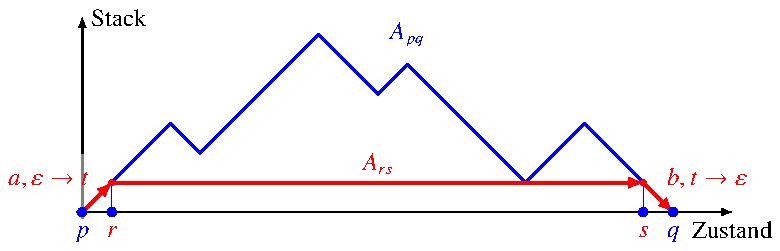
\includegraphics{4-cfg/images/pda-stacknichtleer.pdf}
\end{center}
\caption{Übergänge, die den Stack in keinem Zwischenzustand leeren\label{stacknichtleer}}
\end{figure}

Falls das am Schluss vom Stack entfernte Zeichen nicht das Gleiche ist,
dann muss das $x$ irgendwann im Laufe der Berechnung entfernt worden
sein, und das neue Zeichen $y$ muss auf dem Stack abgelegt worden
sein.
Es gibt also einen Zwischenzustand $r$, in dem der Stack
wieder im selben Zustand wie zu
Beginn der Berechnung ist, wir können dies durch
$A_{pq}\to A_{pr}A_{rq}$ symbolisieren.
Die Abbildung~\ref{stackleer} zeigt diese Situation schematisch.
\begin{figure}
\begin{center}
%\includegraphics[width=0.85\hsize]{images/stack-1.pdf}
%\includegraphics{images/stack-1.pdf}
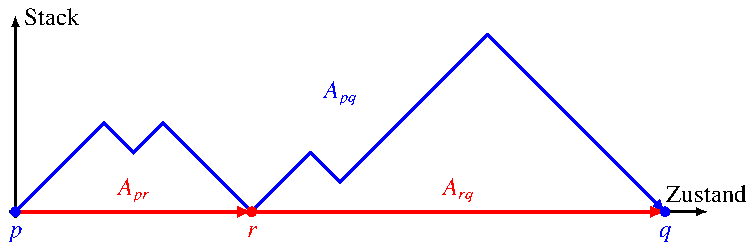
\includegraphics{4-cfg/images/pda-stackleer.pdf}
\end{center}
\caption{Übergänge, die zwischenzeitlich den Stack leeren\label{stackleer}}
\end{figure}

Formal konstruieren wir also eine Grammatik mit Variablen
$V=\{A_{pq}\;|\; p,q\in Q\}$, Startvariable ist $A_{q_0,q_a}$.
Die Menge der Regeln bauen wir wie folgt auf:
\begin{itemize}
\item Für $p,q,r,s\in Q$, $t\in\Gamma$ und $a,b\in\Sigma_{\varepsilon}$:
Falls $\delta(p,a,\varepsilon)$ das Paar $(r,t)$ enthält
und $\delta(s,b,t)$ das Paar $(q,\varepsilon)$, füge die Regel
$A_{pq}\to aA_{rs}b$ hinzu.

Diese Regel besagt, dass Wörter zwischen $p$ und $q$ dadurch gebildet
werden können, dass zunächst ein Zeichen $a$ verarbeitet, und
ein Zeichen $t$ auf den Stack geschrieben wird, dann wird ein Wort
in $A_{rs}$ erzeugt, und zum Schluss das Zeichen $t$ unter
gleichzeitiger Verarbeitung des Zeichens $b$ wieder vom Stack
genommen.

\[
\begin{gathered}
\entrymodifiers={++[o][F]}
\xymatrix{
{p}      \ar[r]^{a,\varepsilon\to t} \ar[d]_{A_{pq}}
	&{r}\ar[d]^{A_{rs}}
\\
{q}
	&{s}\ar[l]^{b,t\to\varepsilon}
}
\end{gathered}
\qquad\rightsquigarrow\qquad A_{pq}\to aA_{rs}b
\]


\item Für drei Zustände $p,q,r\in Q$ füge die Regel 
$A_{pq}\to A_{pr}A_{rq}$ hinzu.
\[
\begin{gathered}
\entrymodifiers={++[o][F]}
\xymatrix{
{p}\ar[dr]^{A_{pr}}\ar[dd]_{A_{pq}}
\\
*+\txt{}
	&{r}\ar[dl]^{A_{rq}}
\\
{q}
}
\end{gathered}
\qquad\rightsquigarrow\qquad A_{pq}\to A_{pr}A_{rq}
\]
\item Für jeden Zustand $p\in Q$ füge die Regel $A_{pp}\to \varepsilon$
hinzu:
\[
\begin{gathered}
\entrymodifiers={++[o][F]}
\xymatrix{
*+\txt{}
	&{p} \ar@(ur,dr)^{A_{pp}}
}
\end{gathered}
\qquad\rightsquigarrow\qquad
A_{pp}\to\varepsilon.
\]
\end{itemize}
Jetzt muss man nur noch zeigen, dass ein Wort $w$ genau dann aus $A_{pq}$
abgeleitet werden kann, wenn es $P$ vom Zustand $p$ mit leerem Stack
in den Zustand $q$ mit leerem Stack bringen kann.


\begin{hilfssatz}\label{apq_generates_x_implies}
Falls $A_{pq}$ das Wort $x$ erzeugt, dann kann $x$ $P$ aus dem Zustand
$p$ mit leerem Stack in den Zustand $q$ mit leerem Stack überführen.
\end{hilfssatz}

\begin{proof}[Beweis von Hilfssatz \ref{apq_generates_x_implies}]
Man kann vollständige Induktion für die Länge der be\-nötigten 
Ableitung $A_{pq}\overset{*}{\Rightarrow} x$ verwenden.

Falls die Ableitung mit nur einem Schritt möglich ist, dann muss
dazu eine Regel der Form $A_{pp}\to\varepsilon$ verwendet werden,
denn dies sind die einzigen Regeln, die auf der rechten Seite
keine Variablen enthalten.

Nehmen wir also an, für Ableitungen der Länge $k$ sei bereits
bekannt, dass sie den Automaten von einem Zustand mit leerem Stack
in einen anderen Zustand mit leerem Stack überführen.

Sei jetzt $A_{pq}\overset{*}{\Rightarrow}x$ eine Ableitung mit $k+1$
Schritten.
Der erste Schritt dieser Ableitung ist entweder eine
Regel der Form $A_{pq}\to aA_{rs}b$ oder $A_{pq}\to A_{pr}A_{rq}$.
Im ersten Fall sagt die Regel, dass $x=ayb$, wobei $y$ ein
Wort ist, welches aus $A_{rs}$ in höchstens $k$ Schritten abgeleitet
werden kann.
Also kann nach Induktionsannahme $y$ den Automaten vom
Zustand $r$ mit leerem Stack in den Zustand $s$ mit leerem Stack
überführen.
Der Übergang von $q$ nach $r$ mit Inputzeichen $a$
legt möglicherweise ein Zeichen $t$ auf den Stack, nach Konstruktion
der Produktionsregeln wird dieses vom Übergang mit Inputzeichen $b$
auch wieder entfernt, so dass der Stack wieder leer ist.

Im zweiten Falls ist nach Induktionsannahme $x=yz$, wobei $y$ den
Automaten vom Zustand $q$ in den Zustand $r$ je mit leerem Stack
überführt, und $z$ ihn von $r$ nach $q$ je mit leerem Stack
führt.

In beiden Fällen folgt, dass $x$ den Automaten von $p$
nach $q$ je mit leerem Stack führen kann.
Damit ist der Induktionsschritt vollzogen, und es folgt, dass
sich jede Ableitung durch Übergänge im Stackautomaten zwischen
Zuständen mit jeweils leerem Stack bilden lassen.
\end{proof}

\begin{hilfssatz}\label{implies_apq_generates_x}
Falls $x$ $P$ aus dem Zustand $p$ mit leerem Stack in den Zustand
$q$ mit leerem Stack überführen kann, dann ist
$A_{pq}\overset{*}{\Rightarrow} x$.
\end{hilfssatz}

\begin{proof}[Beweis von Hilfssatz \ref{implies_apq_generates_x}]
Auch diesen Teil kann man mit vollständiger Induktion beweisen,
diesmal über die Länge der Berechnung.

Die kürzeste mögliche Berechnung hat $0$ Schritte, d.\,h.~sie endet
im gleichen Zustand, in dem sie begonnen hat.
Und tatsächlich enthält die Grammatik die Regel $A_{pp}\to\varepsilon$, 
so dass das leere Wort tatsächlich aus $A_{pp}$ mit leerem
Stack abgeleitet werden kann.

Nehmen wir jetzt an, dass bereits bekannt ist, dass Berechnungen mit
$k$ Schritten, welche $P$ mit dem Input-Wort $w$ vom Zustand $p$
in den Zustand $q$ je mit leerem Stack dazu führen, dass
$A_{pq}\overset{*}{\Rightarrow} x$.

Sei jetzt also eine Berechnung mit Inputwort $x$
mit $k+1$ Schritten gegeben, die $P$ vom Zustand $p$ in den Zustand $q$ 
je mit leerem Stack führt.
Entweder ist der Stack nur ganz zu
Beginn oder ganz am Schluss leer, oder er wird dazwischen einmal
leer.

Im ersten Fall wird ein Symbol $t$ beim ersten Schritt auf den Stack
gelegt, und beim letzten Schritt entfernt.
Es gibt also zwei Zustände
$r$ und $s$ und Übergänge
\[
\entrymodifiers={++[o][F]}
\xymatrix{
p\ar[r]^{a,\varepsilon\to t}
	&r\ar[r]
		&s\ar[r]^{b,t\to\varepsilon}
			&q
}
\]
Die Berechnung, die $P$ von $r$ in $s$ überführt, ist kürzer, und kann
mit leerem Stack durchgeführt werden.
Also ist sie nach Induktionsannahme der Teil $y$ in $x=ayb$ aus
$A_{rs}$ ableitbar.

Im zweiten Fall zerfällt die Berechnung, in der $x$ $P$ von $p$ in
$q$  mit leerem Stack überführt in zwei Teile, die mit Inputwörtern
$y$ und $z$ $p$ in $r$ bzw.~$r$ in $q$ je mit leerem Stack überführen:
\[
\entrymodifiers={++[o][F]}
\xymatrix{
p\ar[r]
	&r\ar[r]
		&q
}
\]
Nach Induktionsannahme ist daher
$A_{pr}\overset{*}{\Rightarrow}y$
$A_{rq}\overset{*}{\Rightarrow}z$, und zusammen mit der Regel
$A_{pq}\to A_{pr}A_{rq}$ der Grammatik auch
$A_{pq}\overset{*}{\Rightarrow} x$
\end{proof}

Damit ist auch der Beweis von Hilfssatz \ref{pda_has_grammar} vollständig.
\end{proof}

\begin{beispiel}
Wir möchten die Theorie dazu verwenden, für den Stackautomaten aus
Abschnitt~\ref{stackbeispiele} für die Sprache
$L=\{\texttt{0}^n\texttt{1}^n\;|\; n\ge 0\}$ eine Grammatik zu finden.
Dazu wandeln wir zunächst den Stackautomaten in die Standardform um, die
wir für die Konstruktion der Grammatik brauchen.
Dazu müssen wir im vertikalen Übergang einen Zwischenzustand einfügen:
\[
\entrymodifiers={++[o][F]}
\xymatrix{
*+\txt{}\ar[r]
	&{q_0}\ar[r]^{\varepsilon,\varepsilon\to{\tt \$}}
		&{q_1} \ar@(ur,dr)^{{\tt 0},\varepsilon\to{\tt 0}}
		    \ar[d]^{\varepsilon,\varepsilon\to x}
\\
*+\txt{}
	&*+\txt{}
		&{q_2}\ar[d]^{\varepsilon,x\to\varepsilon}
\\
*+\txt{}
	&*++[o][F=]{q_a}
		&{q_3}\ar[l]^{\varepsilon,{\tt \$}\to\varepsilon}
		   \ar@(ur,dr)^{{\tt 1},{\tt 0}\to\varepsilon}
}
\]
Die Startvariable der Grammatik ist $A_{q_0q_a}$.
Die Übergänge, die
das Zeichen $\texttt{\$}$ behandeln, führen zu einer Regel
\begin{equation}
A_{q_0q_a}\to \varepsilon A_{q_1q_3}\varepsilon = A_{q_1q_3}.
\label{q0qa}
\end{equation}
Wenn man im Zustand $q_1$ eine $\texttt{0}$ auf den Stack legt, dann
muss man sie auch im Zustand $q_3$ wieder entfernen.
Dieser Prozess gibt Anlass zu einer Regel
\begin{equation}
A_{q_1q_3}\to \texttt{0}\; A_{q_1q_3}\;\texttt{1}
\label{q1q3}
\end{equation}
Man kann aber auch ohne eine $\texttt{0}$ auf dem Stack von
$q_1$ zu $q_3$ gelangen, das führt zu der Regel 
\begin{equation}
A_{q_1q_3}\to \varepsilon\; A_{q_2q_2}\;\varepsilon
\label{q2q2}
\end{equation}
Zusätzlich hat man noch die Regel $A_{q_2q_2}\to\varepsilon$, da 
$A_{q_2q_2}$ nur in (\ref{q2q2}) gebraucht wird, können wir sie
bereits anwenden, und erhalten so die Grammatik.
\begin{align}
A_{q_0q_a}&\to A_{q_1q_3} \tag{\ref{q0qa}}\\
A_{q_1q_3}&\to \texttt{0}\; A_{q_1q_3}\;\texttt{1} \tag{\ref{q1q3}}\\
A_{q_1q_3}&\to \varepsilon\tag{\ref{q2q2}}
\end{align}
Es werden nur noch zwei Variablen verwendet, aber die Startvariable
wird immer in $A_{q_1q_3}$ umgewandelt, man kann sie also auch noch
einsparen.
Schreiben wir $S=A_{q_1q_3}$ bleibt somit als Grammatik
\begin{align}
S&\to \texttt{0}\; S\; \texttt{1}\tag{\ref{q1q3}}\\
S&\to\varepsilon,\tag{\ref{q2q2}}
\end{align}
genau die Grammatik, die wir früher schon für $L$ gefunden haben.
\end{beispiel}


%
% noncfl.tex -- nicht kontextfreie Sprachen
%
% (c) 2019 Prof Dr Andreas Müller, Hochschule Rapperswil
%
\section{Nicht kontextfreie Sprachen}
\rhead{Nicht kontextfreie Sprachen}
Mit einem Stack kann man nur über eine Art von eingegangenen
Zeichen Buch führen.
Möchte man mehrere Zeichen verfolgen,
bräuchte man freien Zugriff auf verschiedene Zähler für jedes
Zeichen.
Eine Maschine mit so vielen Stacks wie Zeichen zur Verfügung
stehen, könnte also auch die Sprache
\[
L=\{ {\tt a}^n {\tt b}^n {\tt c}^n\;|\;n\in\mathbb N\}
\]
erkennen.
Ein ``standard'' Stackautomat kann das jedoch nicht,
in diesem Abschnitt soll gezeigt werden, dass $L$ nicht kontextfrei
ist.

\subsection{Pumping Lemma für kontextfreie Sprachen}
\index{Pumping Lemma!für kontextfreie Sprachen}%
Bei regulären Sprachen ermöglicht das Pumping-Lemma den einfachen
Beweis, dass eine Sprache nicht regulär ist.
Die Grundidee dabei ist,
dass sich in einem endlichen Automaten früher oder später ein
Zustand wiederholen muss, und dass die Schleife zwischen dem ersten
und dem zweiten Auftreten dieses Zustandes beliebig oft durchlaufen
werden kann, um immer wieder neue akzeptable Wörter zu liefern.

Die Äquivalenz von kontextfreien Sprachen mit Sprachen, die von einem
Stackautomaten akzeptiert werden können, suggeriert, dass so etwas
auch für kontextfreie Sprachen möglich sein sollte.
Stackautomaten
wurden aber grundsätzlich als nicht deterministische Automaten
konstruiert, wo die Argumente, die das Pumping Lemma für reguläre
Sprachen geliefert haben, nicht direkt anwendbar sind.
Wir verwenden
daher nicht einen Stackautomaten, sondern direkt die Grammatik, um
das Pumping Lemma herzuleiten.

\begin{figure}
\begin{center}
\includegraphics[width=0.35\hsize]{images/cfg-1}
\end{center}
\caption{Parse Tree für die Erzeugung des Wortes $uvxyz$ aus der
Startvariablen $S$.\label{cfg-tree-1}}
\end{figure}
\begin{figure}
\begin{center}
\begin{tabular}{cc}
\includegraphics[width=0.35\hsize]{images/cfg-2}&%
\includegraphics[width=0.35\hsize]{images/cfg-3}\\
\end{tabular}
\end{center}
\caption{Parse Tree für das aufgepumpte Wort $uv^2xy^2z$ (links) und das
abgepumpte Wort $uxz$ (rechts).\label{cfg-tree-2}}
\end{figure}

Ist ein Wort $w\in L(G)$ genügend lang, gibt es auch lange Pfade im
Ableitungsbaum.
Bei Verwendung der Chomsky-Normalform ist die 
Tiefe des Baumes im besten Fall $\log_2 |w|$, im schlimmsten Fall $|w|-1$.
Ist $|w|>2^{|V|}$, muss mindestens eine
Variable auf einem Ast des Baumes zweimal verwendet werden\footnote{
Innerhalb des Baumes werden genau $|w|-1$ Regeln der
Form $A\to BC$ angewendet.
Trotzdem reicht es nicht, $|w|-1>|V|$ zu verlangen, weil die
zweimal verwendete Variable nicht auf dem gleichen Ast des
Baumes zu sein braucht.
Für die Durchführung des Argumentes
brauchen wir aber, dass wir die beiden Vorkommnisse der Variablen
über Ableitungsregeln verbinden können.}.
Sei $A$ die unterste Variable im Ableitungsbaum, die wiederholt
wird (Abbildung~\ref{cfg-tree-1}).
Es erzeugt ein Wort $x$.
Das nächsthöhere Vorkommen von $A$
erzeugt dagegen ein Wort, welches aus drei Teilen besteht:
$vxy$, die Länge dieses Wortes ist $\le N$.
Für das ganze Wort fehlen
noch die Teile, die von Regeln ``weiter oben'' im Ableitungsbaum
erzeugt werden, also $w=uvxyz$.
Da die beiden Vorkommnisse von $A$ veschieden sind, muss mindestens
eines der Teilwörter $v$ und $y$ nicht leer sein, also $|vy|>0$
Indem man den Teil des Ableitungsbaumes
zwischen den Vorkommnissen von $A$ repliziert, kann man jetzt die
Wörter $uv^kxy^kz$ bilden, die alle auch mit der Grammatik $G$ 
abgeleitet werden können, also zu $L(G)$ gehören (Abbildung~\ref{cfg-tree-2}).
Damit haben wir folgenden Satz bewiesen:

\begin{satz}[Pumping Lemma für kontextfreie Sprachen]
\index{Pumping Lemma!für kontextfreie Sprachen}%
\index{pumping length!für kontextfreie Sprachen}%
Sei $L$ eine kontextfreie Sprache, dann gibt es ein Zahl $N$, die pumping
length, so dass jedes Wort $w\in L$ mit $|w|\ge N$ zerlegt werden
kann in fünf Teile $w=uvxyz$
\begin{compactenum}
\item
$|vy|>0$,
\item
$|vxy|\le N$ und
\item
$uv^kxy^kz\in L$ für alle $k\in\mathbb N$.
\end{compactenum}
\end{satz}

\subsection{Beispiele nicht kontextfreier Sprachen}
\subsubsection{Die Sprache $L=\{a^nb^nc^n\,|\,n\in\mathbb N\}$.}
\begin{figure}
\begin{center}
%\includegraphics[width=\hsize]{images/pl-5}\\%
\includegraphics{images/pl-5}\\%
\smallskip
%\includegraphics[width=\hsize]{images/pl-6}\\%
\includegraphics{images/pl-6}\\%
\smallskip
%\includegraphics[width=\hsize]{images/pl-7}\\%
\includegraphics{images/pl-7}\\%
\smallskip
%\includegraphics[width=\hsize]{images/pl-8}%
\includegraphics{images/pl-8}%
\end{center}
\caption{Pumping Lemma für kontextfreie Sprachen angewandt auf das 
Wort ${\tt a}^N{\tt b}^N{\tt c }^N\in L$, wobei $N$ die pumping length
von $L$ ist.
Da $w$ lang genug ist, gibt es eine Zerlegung 
$w=uvxyz$ (2.~Zeile).
Abpumpen (3.~Zeile) und Aufpumpen (4.~Zeile) des
Wortes führt zu Wörtern, die nicht mehr in $L$ liegen.\label{pumpingcfgimage}}
\end{figure}

Die Sprache $L=\{a^nb^nc^n\;|\;n\in\mathbb N\}$ ist nicht kontextfrei.
Wir verwenden das Pumping Lemma für kontextfreie Sprachen.
Dazu nehmen wir zunächst an, die Sprache $L$ sei kontextfrei.
Dann besagt das Pumping Lemma, dass es eine Zahl $N$ gibt, so dass
Wörter mit Länge mindestens $N$ besondere Eigenschaften haben.
Als solches langes Wort nehmen wir $w=a^Nb^Nc^N$.
Nach dem Pumping Lemma gibt es eine Zerlegung in fünf Teile
$w=uvxyz$, wobei der mittlere Teil nicht zu lang ist:
$|vxy|\le N$ (Abbildung~\ref{pumpingcfgimage}).
Insbesondere enthält $|vxy|$ höchstens zwei
Arten von Zeichen, denn es ist zu kurz, die $N$ $b$s in der Mitte
von $w$ zu überspannen.
Beim Aufpumpen zu $uv^kxy^kz$ nimmt also
die Zahl dieser beiden Zeichen zu, nicht jedoch die Zahl des nicht
in $vxy$ enthaltenen Zeichens.
Damit kann $uv^kxy^kz$ nicht mehr in $L$ sein, obwohl das
Pumping Lemma dies behauptet.
Aus diesem Widerspruch folgt, dass $L$ nicht kontextfrei sein kann.


%
% realworldparser.tex
%
% (c) 2019 Prof Dr Andreas Müller, Hochschule Rapperswil
%
\rhead{Praktische Parser}
\section{Real World Parser}
\subsection{Deterministische Parser}
Kontextfreie Sprachen können von einem nichtdeterministischen
Stackautomaten analysiert werden. Ein deterministischer Algorithmus mit
kubischer Laufzeit ist verfügbar. Doch kubische Laufzeit ist bei grossem
Input immer noch sehr gross, eine Verdoppelung der Inputgrösse hat eine
Verachtfachung der Laufzeit zur Folge. 
Für praktische Zwecke der Syntaxanalyse
zum Beispiel in einem Compiler wird daher ein Verfahren benötigt, welches
Wörter deterministisch in linearer Zeit erkennen kann.

Leider ist das in voller Allgemeinheit nicht möglich. Daher wurden Parser-Techniken
erfunden, welche deterministisch und in linearer Laufzeit Sprachen erkennen,
deren Grammatiken zusätzliche Eigenschaften haben. Natürlich sollen diese
Techniken möglichst nicht mehr als einen Stackautomaten benötigen, den Input
von links nach rechts lesen und wenn möglich laufend die Informationen ausgeben,
die zum Beispiel für die Erzeugung von Code in einem Compiler benötigt wird.
Eine besonders wichtige Familie von Parsern sind die $LR(k)$-Parser.
Ihr Name leitet sich aus der Tatsache ab, dass der Input von Links gelesen wird,
dabei Rechtsreduktionen durchgeführt werden und höchstens $k$ Inputzeichen
vorausgelesen werden müssen, um zu entscheiden, welche Produktionsregel der
Grammatik für die Reduktion angewendet werden soll.

Der nicht deterministische Stackautomat ist so konstruiert worden, dass er aus
der Startvariablen auf dem Stack durch Anwendung der Produktionsregeln 
ein Wort konstruiert. Das Resultat der bereits angewendeten Regeln
liegt auf dem Stack. Sobald zuoberst auf dem Stack ein Terminalsymbol auftaucht,
kann es mit dem nächsten Zeichen des Input verglichen und bei Übereinstimmung
gelesen werden. Das Input-Wort wird akzeptiert, wenn der Stack und der Input
gleichzeitig leer werden. Nicht deterministisch ist jeweils die Auswahl der
Produktionsregel.

Der Prozess wird also sozusagen vom Orakel gesteuert,
welches die Produktionsregeln vorschlägt. Der Input spielt dabei gar keine
Rolle, man hat es nur den guten Eigenschaften des Orakels zu verdanken,
dass der Input auf den vom Prozess erzeugten String passt.

\subsection{Shift-Reduce}
\index{shift-reduce Parser}%
Ein deterministischer Prozess muss stattdessen vom Input kontrolliert werden.
Das Input-Zeichen oder der aktuelle Stackinhalt müssen bestimmen, was
als nächstes zu geschehen hat. Wie das erreicht werden könnte, kann man am
Beispiel der Sprache $L=\{\texttt{0}^n\texttt{1}^n|n> 0\}$ erahnen, welche die
Grammatik
\begin{align}
w&\rightarrow \texttt{0}\;w\;\texttt{1}\tag{1}\\
&\rightarrow \texttt{01}\tag{2}
\end{align}
hat. Ein Parser könnte bei der Analyse des Wortes $\texttt{000111}$ wie folgt vorgehen.
Er schiebt Zeichen um Zeichen vom Input auf den Stack. Sobald
er erkennt, dass auf dem Stack eine Folge von Zeichen liegt, die auf die rechte
Seite einer Regel passt, wendet er die Regel an, reduziert das Wort zu einer
Variablen und legt das Resultat auf den Stack. Dies ist in Tabelle \ref{shiftreduce}
dargestellt.

\begin{table}[H]
\begin{center}
\begin{tabular}{|r|l|l|}
\hline
Input&Stack&Operation\\
\hline
$\texttt{000111}$&&Schiebe\\
$\texttt{00111}$&$\texttt{0}$&Schiebe\\
$\texttt{0111}$&$\texttt{00}$&Schiebe\\
$\texttt{111}$&$\texttt{000}$&Schiebe\\
$\texttt{11}$&$\texttt{0001}$&Reduziere mit Regel 2\\
$\texttt{11}$&$\texttt{00}w$&Schiebe\\
$\texttt{1}$&$\texttt{00}w\texttt{1}$&Reduziere mit Regel 1\\
$\texttt{1}$&$\texttt{0}w$&Schiebe\\
&$\texttt{0}w\texttt{1}$&Reduziere mit Regel 1\\
&$w$&\\
\hline
\end{tabular}
\end{center}

\caption{Vorgehen eins Shift-Reduce-Parser am Beispiel der Sprache $L=\{\texttt{0}^n\texttt{1}^n|n>0\}$
\label{shiftreduce}}
\end{table}
Offenbar konnte das Wort durch systematisches Anwenden der Regeln aus dem Input
auf die Startvariable zurückgeführt werden.
In der dritten Spalte kann man nachlesen, wie der Parse-Tree aufgebaut ist,
die Regeln treten dabei in der Reihenfolge ``von unten nach oben'' auf.

Ein solcher Parser heisst eine Shift-Reduce-Parser, er baut den Parse-Tree von unten
her (bottom-up) auf, und operiert offenbar vollständig deterministisch.
Er kann jedoch nicht mit einem Stackautomaten implementiert werden,
weil Die Aufforderung ``Schaue nach, ob die obersten $n$ Elemente auf dem Stack
auf die rechte Seite einer Regel passen'', ist für bei einem Stack nicht
durchführbar. Man kann immer nur das oberste Element einsehen.

\subsection{\texorpdfstring{$LR(0)$}{LR(0)}-Elemente}
\index{LR(0)-Element@$LR(0)$-Element}%
Ein Stackautomat kann sich nur dann an den den Stackinhalt unterhalb des obersten
Stackelementes erinnern, wenn er diese Information in Zuständen codieren kann.
Im Beispiel kamen folgende relevanten Stackinhalte vor 
\[
\texttt{0}
\qquad
\texttt{01}
\qquad
\texttt{0}w
\qquad
\texttt{0}w\texttt{1}
\]
Die Inhalte $\texttt{01}$ und $\texttt{0}w\texttt{1}$ haben die Anwendung einer wohl bestimmten
Reduktionsregel
hervorgerufen, die anderen zwei waren nur Vorstufen dazu.
Fasst man diese Wörter
zusammen als Namen der Zustände, können wir den Parse-Prozess wie in
Tabelle \ref{lrelemente} durchführen.
\begin{table}[H]
\begin{center}
\begin{tabular}{|r|l|c|l|l|}
\hline
Input&Stack&Zustand&Reduktion&Operation\\
\hline
$\texttt{000111}$
	&
		&&&Schiebe $\texttt{0}$\\
$\texttt{00111}$
	&$\boxed{\texttt{0}}$
		&$\boxed{\texttt{0}}$&&Schiebe $\texttt{0}$\\
$\texttt{0111}$
	&$\boxed{\texttt{0}}\,\boxed{\texttt{0}}$
		&$\boxed{\texttt{0}}$&&Schiebe $\texttt{0}$\\
$\texttt{111}$
	&$\boxed{\texttt{0}}\,\boxed{\texttt{0}}\,\boxed{\texttt{0}}$
		&$\boxed{\texttt{0}}$&&Schiebe $\texttt{1}$\\
$\texttt{11}$
	&$\boxed{\texttt{0}}\,\boxed{\texttt{0}}\,\boxed{\texttt{0}}\,\boxed{\texttt{01}}$
		&$\boxed{\texttt{01}}$&&Reduziere, Regel 2\\
$\texttt{11}$
	&$\boxed{\texttt{0}}\,\boxed{\texttt{0}}$
		&$\boxed{\texttt{0}}$&$w$&Schiebe $w$\\
$\texttt{11}$
	&$\boxed{\texttt{0}}\,\boxed{\texttt{0}}\,\boxed{\texttt{0}w}$
		&$\boxed{\texttt{0}w}$&&Schiebe $\texttt{1}$\\
$\texttt{1}$
	&$\boxed{\texttt{0}}\,\boxed{\texttt{0}}\,\boxed{\texttt{0}w}\,\boxed{\texttt{0}w\texttt{1}}$
		&$\boxed{\texttt{0}w\texttt{1}}$&&Reduziere, Regel 1\\
$\texttt{1}$
	&$\boxed{\texttt{0}}$
		&$\boxed{\texttt{0}}$&$w$&Schiebe $w$\\
$\texttt{1}$
	&$\boxed{\texttt{0}}\,\boxed{\texttt{0}w}$
		&$\boxed{\texttt{0}w}$&&Schiebe $\texttt{1}$\\
	&$\boxed{\texttt{0}}\,\boxed{\texttt{0}w}\,\boxed{\texttt{0}w\texttt{1}}$
		&$\boxed{\texttt{0}w\texttt{1}}$&&Reduziere, Regel 1\\
	&
		&$\boxed{\phantom{\texttt{0}}}$&$w$&zum Endzustand\\
\hline
\end{tabular}
\end{center}

\caption{Shift-Reduce mit $LR(0)$-Elementen\label{lrelemente}}
\end{table}
Der Automat legt also immer seinen neuen Zustand zuoberst auf den
Stack, behält aber die alten Zustände. Der Name des Zustandes ist
die teilweise gelesene rechte Seite einer Regel, man kann also aus
dem Namen des Zustandes auch ablesen, welche Regeln für den nächsten
Reduktionsschritt in Frage kommen könnten.

Wir markieren innerhalb einer Regel die ``Position des Lesers'' mit
einem Punkt, wir erhalten dann aus der Grammatik
\begin{align}
\cdot\;\texttt{0}\;w\;\texttt{1}&\leftarrow w\tag{1}\\
\texttt{0}\;\cdot\;w\;\texttt{1}&\leftarrow w\tag{1}\\
\texttt{0}\;w\;\cdot\;\texttt{1}&\leftarrow w\tag{1}\\
\texttt{0}\;w\;\texttt{1}\;\cdot&\leftarrow w\tag{1}\\
\cdot\;\texttt{0}\;\texttt{1}&\leftarrow w\tag{2}\\
\texttt{0}\;\cdot\;\texttt{1}&\leftarrow w\tag{2}\\
\texttt{0}\;\texttt{1}\;\cdot&\leftarrow w\tag{2}
\end{align}
Der Teil links vom $\cdot$ zeigt an, was bereits gelesen wurde,
rechts davon findet
man die Zeichen, die als nächste gelesen werden dürfen.
Befindet sich $\cdot$
am Ende des Wortes, kann die Reduktion agewendet werden.
Man nennt die so erweiterten
Produktionsregeln die {\em $LR(0)$-Elemente}.

\subsection{Übergangsfunktion des \texorpdfstring{$LR(0)$}{LR(0)}-Parsers}
Wenn eine Reduktionsregel angewendet werden kann, werden so viele Elemente
aus dem Stack entfernt, wie die rechte Seite der Regel Zeichen hat. Das
neue oberste Zeichen auf dem Stack ist der letzte Zustand des Automaten
bevor die jetzt reduzierten Zeichen gelesen wurden. Dieser Zustand
bestimmt zusammen mit dem Reduktionsresultat den nächsten Zustand
des Automaten.

Es gilt jetzt zu überprüfen, dass diese Operationen tatsächlich mit
Hilfe eines Stackautomaten durchführbar sind. Die einfachste ist natürlich
die Shift-Ope\-ration. Da diese jedoch abhängig ist vom aktuellen Element zuoberst
auf dem Stack, braucht es dafür zwei Schritte:
\[
\boxed{\texttt{0}}\xrightarrow{\texttt{0},\scalebox{0.7}{\boxed{\texttt{0}}$\rightarrow$\boxed{\texttt{0}}}}\cdot
\xrightarrow{\varepsilon,\varepsilon\rightarrow\scalebox{0.7}{\boxed{\texttt{0}}}}\boxed{\texttt{0}}
\]
oder
\[
\boxed{\texttt{0}}\xrightarrow{\texttt{1},\scalebox{0.7}{\boxed{\texttt{0}}$\rightarrow$\boxed{\texttt{0}}}}\cdot
\xrightarrow{\varepsilon,\varepsilon\rightarrow\scalebox{0.7}{\boxed{\texttt{01}}}}\boxed{\texttt{01}},
\]
in beiden Fällen wird ein neuer Zwischenzustand benötigt, symbolisiert mit dem Zeichen
`$\cdot$'.

Die Reduktion mit der Regel 2 muss zwei Zustände vom Stack entfernen.
Wenn anschliessend der Zustand $\boxed{\texttt{0}}$ auf dem Stack liegt, ist der
nächste Zustand $\boxed{\texttt{0}w}$. Dies kann man mit folgenden Übergängen
realisieren:
\[
\boxed{\texttt{01}}
\xrightarrow{\varepsilon,\scalebox{0.7}{\boxed{\texttt{01}}}\to\varepsilon}
\cdot
\xrightarrow{\varepsilon,\scalebox{0.7}{\boxed{\texttt{0}}}\to\varepsilon}
\cdot
\xrightarrow{\varepsilon,\scalebox{0.7}{\boxed{\texttt{0}}}\to\scalebox{0.7}{\boxed{\texttt{0}}}}
\cdot
\xrightarrow{\varepsilon,\varepsilon\to\scalebox{0.7}{\boxed{\texttt{0}w}}}
\boxed{\texttt{0}w}
\]
Analog kann die Reduktion mit der Regel 1 durchgeführt werden:
\[
\boxed{\texttt{0}w\texttt{1}}
\xrightarrow{\varepsilon,\scalebox{0.7}{\boxed{\texttt{0}w\texttt{1}}}\to\varepsilon}
\cdot
\xrightarrow{\varepsilon,\scalebox{0.7}{\boxed{\texttt{0}w}}\to\varepsilon}
\cdot
\xrightarrow{\varepsilon,\scalebox{0.7}{\boxed{\texttt{0}}}\to\varepsilon}
\cdot
\xrightarrow{\varepsilon,\scalebox{0.7}{\boxed{\texttt{0}}}\to\scalebox{0.7}{\boxed{\texttt{0}}}}
\cdot
\xrightarrow{\varepsilon,\varepsilon\to\scalebox{0.7}{\boxed{\texttt{0}w}}}
\boxed{\texttt{0}w}
\]
Wir können diese Übergänge etwas einfacher schreiben, wenn wir in der
Beschriftung der Pfeile erlauben, mehrere Operationen zusammenzufassen.
Die Shift-Ope\-rationen werden dann zu
\begin{gather*}
\boxed{\texttt{0}}\xrightarrow{\texttt{0},\scalebox{0.7}{\boxed{\texttt{0}}$\rightarrow$\boxed{\texttt{0}}\,\boxed{\texttt{0}}}}\boxed{\texttt{0}}
\\
\boxed{\texttt{0}}\xrightarrow{\texttt{1},\scalebox{0.7}{\boxed{\texttt{0}}$\rightarrow$\boxed{\texttt{0}}\,\boxed{\texttt{01}}}}\boxed{\texttt{01}}
\end{gather*}
die Reduktionsoperationen zu
\begin{gather*}
\boxed{\texttt{01}}
\xrightarrow{\varepsilon,\scalebox{0.7}{\boxed{\texttt{0}}\,\boxed{\texttt{01}}}\to\varepsilon}
\cdot
\xrightarrow{\varepsilon,\scalebox{0.7}{\boxed{\texttt{0}}}\to\scalebox{0.7}{\boxed{\texttt{0}}\,\boxed{\texttt{0}w}}}
\boxed{\texttt{0}w}
\\
\boxed{\texttt{0}w\texttt{1}}
\xrightarrow{\varepsilon,\scalebox{0.7}{\boxed{\texttt{0}}\,\boxed{\texttt{0}w}\,\boxed{\texttt{0}w\texttt{1}}}\to\varepsilon}
\cdot
\xrightarrow{\varepsilon,\scalebox{0.7}{\boxed{\texttt{0}}}\to\scalebox{0.7}{\boxed{\texttt{0}}\,\boxed{\texttt{0}w}}}
\boxed{\texttt{0}w}
\end{gather*}
In diesem einfachen Bespiel gibt es nur eine Möglichkeit für den zweiten
Schritt, in einer komplexeren Grammatik könnte nach der Reduktion jedoch
eine Vielzahl anderer Zustände auf dem Stack zurückbleiben, so dass je
nach vorherigem Zustand $q$ weitere Übergänge der Form
\[
\cdot\xrightarrow{\varepsilon,q\to q q'}q'
\]
hinzugenommen werden müssen. Es folgt, dass obiger $LR(0)$-Parser mit
Hilfe eines Stackautomaten implementiert werden kann.

\subsection{Parser-Tabellen}
Da gezeigt wurde, dass der Beispiel-$LR(0)$-Parser in einem Stackautomaten
implementiert werden kann, kann die Übergangsfunktion mit Hilfe
einer Tabelle codiert werden. Die Zeilen dieser Tabelle sind die
Zustände, also die $LR(0)$-Elemente. In den Spalten müssen die
Schiebe- und Reduktions-Schritte codiert sein. In einem Zustand
entscheidet man sich immer entweder für einen Reduktionsschritt
unabhängig vom Input, oder für eine Schiebeoperation, wobei
nicht alle Input-Zeichen akzeptabel sind, und verschiedene Eingabezeichen
zu verschiedenen Ausgabezuständen führen können. Das Beispiel
$L=\{\texttt{0}^n\texttt{1}^n|n>0\}$ führt auf Tabelle \ref{parsetable}.
\begin{table}[H]
\begin{center}
\begin{tabular}{|c|c|cc|c|}
\hline
Zustand&$LR(0)$-Element&$0$&$1$&$w$\\
\hline
0&$\boxed{\phantom{\texttt{0}}}$&s1&&\\
1&$\boxed{\texttt{0}}$&s1&s3&4\\
2&$\boxed{w}$&&&\\
3&$\boxed{\texttt{01}}$&r2&r2&\\
4&$\boxed{\texttt{0}w}$&&s5&\\
5&$\boxed{\texttt{0}w\texttt{1}}$&r1&r1&\\
\hline
\end{tabular}
\end{center}

\caption{Parsertabelle für $L=\{\texttt{0}^n\texttt{1}^n|n>0\}$\label{parsetable}}
\end{table}
Die Tabelle ist wie folgt zu lesen. In Spalten 3 und 4 wird jeweils
angegeben, was für eine Aktion ausgeführt werden soll, wenn das
Zeichen $\texttt{0}$ bzw.~$\texttt{1}$ vom Input gelesen wird. Ein s$n$ bedeutet, dass
eine Schiebeoperation ausgeführt wird, und anschliessend in den
Zustand $n$ gewechselt wird. Dagegen bedeutet r$n$,
dass die Reduktionsregel mit der Nummer $n$ angewendet wird.
Dazu gehören folgende Schritte:
\begin{enumerate}
\item
Entferne so viele Elemente vom Stack, wie die rechte Seite der angewendeten
Regel lang ist.
\item
Bestimme den Zustand, der durch das oberste Element auf dem Stack
angezeigt wird.
\item
Bestimme in der eben bestimmten Zeile unter dem Resultat der Reduktion,
welches der nächste Zustand ist.
\item
Lege diesen Zustand zuoberst auf den Stack.
\end{enumerate}
\index{Bison}%
\index{Yacc}%
Die Konstruktion der Parsertabellen ist aufwendig und fehlerträchtig,
doch stehen dafür Softwarewerkzeuge zur Verfügung, zum Beispiel
der Parser-Generator Bison.

\subsection{Konflikte}
\index{Konflikt}%
Diese Art von Parser kann funktionieren, wenn jederzeit klar ist, ob
geschoben werden kann, oder ob eine Reduktion erfolgen soll.
Sind mehrere Operationen möglich, spricht man von einem Konflikt.
\subsubsection{Reduce-Reduce Konflikt}
\index{Konflikt!reduce-reduce}%
In der folgenden Grammatik ist nicht klar, welche der beiden Reduktionsregeln
angewendet werden soll
\begin{align*}
A&\rightarrow \texttt{01}\\
B&\rightarrow \texttt{01}
\end{align*}

\subsubsection{Shift-Reduce Konflikt}
\index{Konflikt!shift-reduce}%
In der folgenden Grammatik ist nach dem Lesen einer $1$ nicht klar
\begin{align*}
A&\rightarrow \texttt{1}\tag{1}\\
A&\rightarrow \texttt{1}\,A\tag{2}
\end{align*}
ob man die Regel (1) anwenden soll (Reduce), oder ob man
in der Hoffnung, irgendwann ein $A$ zu finden, weiterlesen
soll. Diese Frage kann offenbar nur dadurch entschieden werden, dass
man vorausschaut. Dies ist in einem $LR(0)$-Parser nicht erlaubt.
Formuliert man obige Grammatik jedoch mit den Regeln
\begin{align*}
A&\rightarrow \texttt{1}\tag{1}\\
A&\rightarrow A\,\texttt{1}\tag{2}
\end{align*}
kann die Regel (1) jederzeit angewendet werden, der Konflikt ist
weggefallen. 

\section{Real existierende Parser}
Parsergeneratoren wie Yacc oder Bison erweitern die gegebene Grammatik
selb\-ständig um zusätzliche Symbole, die ihnen helfen, das Ende
des Input oder des Stack zu erkennen. Sie fügen dazu eine
Regel
\[
\text{\$accept}\rightarrow S\; \text{\$end}
\]
hinzu. Wenn also am Ende des Input alles auf die Variable $S$ reduziert
werden konnte, liegt offenbar ein Wort vor, welches akzeptiert werden
muss.

\section{Arithmetische Ausdrücke}
\index{expression-term-factor Grammatik}%
\index{Ausdrücke!arithmetische}%
Hier soll an Hand einer Beispiel-Grammatik gezeigt werden, wie ein 
von Bison erzeugter Parser einen arithmetischen Ausdruck
erkennt. Wir verwenden die Grammatik:
\begin{align}
\textsl{expr}&\rightarrow \textsl{term}\tag{2}\\
\textsl{expr}&\rightarrow \textsl{expr}\;\text{'{\tt +}'}\;\textsl{term}\tag{3}\\
\textsl{expr}&\rightarrow \textsl{expr}\;\text{'{\tt -}'}\;\textsl{term}\tag{4}\\
\textsl{term}&\rightarrow \textsl{factor}\tag{5}\\
\textsl{term}&\rightarrow \textsl{term}\;\text{'{\tt *}'}\;\textsl{factor}\tag{6}\\
\textsl{term}&\rightarrow \textsl{term}\;\text{'{\tt /}'}\;\textsl{factor}\tag{7}\\
\textsl{factor}&\rightarrow\text{'{\tt (}'}\;\textsl{expr}\;\text{'{\tt )}'}\tag{8}\\
\textsl{factor}&\rightarrow\textsl{number}\tag{9}\\
\textsl{number}&\rightarrow\textsl{number}\;\textsl{digit}\tag{10}\\
\textsl{number}&\rightarrow\textsl{digit}\tag{11}\\
\textsl{digit}&\rightarrow\text{'{\tt 0}'}\tag{12}\\
\vdots&\qquad\vdots\notag\\
\textsl{digit}&\rightarrow\text{'{\tt 9}'}\tag{21}
\end{align}
Die Nummerierung der Regeln bezieht sich auf die später gezeigten Regeln
der von Bison erzeugten Parsetabellen. Damit diese Grammatik in einem
Programm einfach demonstriert werden kann ist es sinnvoll, ein Endzeichen
für die arithmetischen Ausdrücke einzuführen. Wir fügen zu diesem
Zweck die Regel 
\begin{equation}
\textsl{exprline}\rightarrow \textsl{expr}\;\text{'{\tt $\setminus$n}'}
\tag{1}
\end{equation}
hinzu. Bison fügt dann seinerseits eine Regel mit der Nummer 0 hinzu, so ergibt
sich folgende Grammatik in Bisons Schreibweise:
\verbatiminput{4-cfg/bison/bisongrammar.txt}
Man kann Bison nicht nur mit einer Kommandozeilenoption dazu bringen, diese
Grammatik im Klartext auszugeben, er zeigt auch die erzeugten Parsetabellen
an. Exemplarisch soll dargestellt werden, wie Zustand 14 verarbeitet
wird:
\verbatiminput{4-cfg/bison/state14.txt}
Das zugehörige $LR(0)$-Element beginnt also mit \text{term}. Die Zeichen
`{\tt *}' und `{\tt /}' lösen jeweils eine Schiebeoperation aus, andernfalls
wird mit Hilfe der Regel 2 reduziert.



